\documentclass[submission,nolinenumbers]{esj}
\usepackage{amsmath,amssymb,amsthm,booktabs,enumitem,graphicx,float,tabularx,array,ragged2e}
\newcolumntype{Y}{>{\RaggedRight\arraybackslash}X}
\setlength{\emergencystretch}{2em}
\newcommand{\wrap}{\operatorname{wrap}}
\newcommand{\R}{\mathbb R}
% Generated from results.json; do not hand edit.
\newcommand{\TauMean}{18.052}
\newcommand{\TauSD}{1.006}
\newcommand{\TauTheory}{0.995}
\newcommand{\GammaMean}{0.346}
\newcommand{\AlphaMean}{0.798}
\newcommand{\GammaSD}{0.078}
\newcommand{\AlphaSD}{0.050}
\newcommand{\ChiMean}{0.5994}
\newcommand{\ChiSD}{0.0137}
\newcommand{\NoisyChi}{0.3356}
\newcommand{\NormalCoverage}{94.85\%}
\newcommand{\TCoverage}{95.00\%}
\newcommand{\NoisyCoverage}{2.35\%}
\newcommand{\BootCoverage}{95.00\%}
\newcommand{\BootCount}{57}
\newcommand{\RobustWindow}{0.737}
\newcommand{\PossibleWindow}{0.953}
\newcommand{\ChirpMean}{18.211}
\newcommand{\ChirpSD}{1.511}
\newcommand{\CleanMixRMSE}{0.029}
\newcommand{\MixedRMSE}{0.567}
\newcommand{\MSEAdd}{0.0019065}
\newcommand{\MSEInstant}{0.0020171}
\newcommand{\MSEExcluded}{0.0020625}
\newcommand{\MSEDelay}{0.0004147}
\newcommand{\MSEInclusive}{0.0004183}
\newcommand{\CleanTenRmse}{0.062}
\newcommand{\CleanTenKappa}{1.958}
\newcommand{\MixZeroRmse}{0.355}
\newcommand{\MixZeroKappa}{3.135}
\newcommand{\DriveZeroRmse}{0.332}
\newcommand{\DriveZeroKappa}{2.833}
\newcommand{\MixdriveZeroRmse}{0.557}
\newcommand{\MixdriveZeroKappa}{4.833}
\newcommand{\FalseConst}{20}
\newcommand{\FalseFourier}{0}
\newcommand{\AltGate}{0.07602}
\newcommand{\AltConst}{0.08154}
\newcommand{\AltFourier}{0.04252}


\newcommand{\Dj}{D_j}
\newcommand{\Di}{D_i}
\newcommand{\Tij}{T_{ij}}
\newcommand{\Bij}{B_{ij}}
\newcommand{\Om}{\Omega}
\newcommand{\tauij}{\tau_{ij}}
\newcommand{\etac}{\eta}
\newcommand{\Delt}{\Delta}
\newcommand{\psiw}{\psi}
\newcommand{\Bmap}{\mathcal{B}}
\newcommand{\EA}{\mathrm{E}_A}
\newcommand{\Content}{C}
\newcommand{\epsU}{\varepsilon_u}
\newcommand{\epsD}{\varepsilon_d}
\DeclareMathOperator{\im}{im}
\DeclareMathOperator{\rank}{rank}
\DeclareMathOperator{\Ker}{ker}

\articletype{Research Article}\volume{0}\issue{0}\pubyear{2026}\firstpage{1}
\articledoi{}\received{4 October 2026}
\title{Phase-Gated Interregional Transfer: Single-Band Identifiability, Reciprocal Projection, and Completion Latency}
\shorttitle{Phase-gated transfer and completion latency}\shortauthors{Abdelgalil}
\author[1,*]{Karem Abdelgalil}\affil[1]{Independent Researcher, Cairo, Egypt}
\corresp{Karem Abdelgalil, \href{mailto:kahmed.math.coder@gmail.com}{kahmed.math.coder@gmail.com}}

\begin{abstract}
Single-band carrier phase confounds conduction delay with transfer phase, while a receptive gate controls content amplitude. We formulate a calibrated complex Gaussian observation model and a retarded translation operator to separate parameter identification, projected delivery, threshold completion, and reciprocal return. A carrier-plus-gain observation identifies two effective offsets but leaves a one-dimensional parameter ridge. Two frequencies with shared transfer phase and an informative gain scan remove this local ambiguity on a calibrated phase branch. Nonzero item projection gives a modeled sender-dependent contribution, without ensuring threshold crossing. Reciprocal map products determine which content can return; independently timed echoes supply constraints unavailable from stationary phase. An invariant positive channel gives an explicit round-trip waiting time, while general stable channels permit rotation, cancellation, and transient crossings. A Lyapunov bound extends finite crossing certification to stable non-normal loops. A delayed-network extension derives item-specific supported-route arrival, cancellation-aware threshold bounds, and a dispersion bound while exposing conduction--processing ambiguity. Complement factorial contrasts and a Gaussian readout specify when interaction innovation carries discriminative information. Excitation limits which translation errors the stated learning rule can repair. Fixed-seed synthetic checks include parameter recovery, interval diagnostics, and paired prediction comparisons. Public datasets offer complementary component tests, but no inspected resource establishes the complete joint model. Neural and behavioral validation remains open.
\end{abstract}

\keywords{dictionary translation; conduction delay; phase connectivity; structural identifiability; reciprocal communication; communication subspace; completion latency; interaction rank}

\setlength{\textfloatsep}{6pt plus 2pt minus 2pt}
\setlength{\floatsep}{6pt plus 2pt minus 2pt}
\setlength{\intextsep}{6pt plus 2pt minus 2pt}
\newtheorem{conjecture}{Conjecture}
\begin{document}\maketitle

\section{Introduction and inferential scope}\label{sec:intro}
Communication-through-coherence proposes that phase can change how effectively one population drives another \citep{fries2015,bastos2015}. A communication subspace is the small set of source patterns that a downstream area actually reads \citep{semedo2019}. Access accounts separate local processing from report \citep{dehaene2006}. Recurrent-processing accounts separate experience from report \citep{lamme2006}. Coherence can follow a message rather than cause it \citep{schneider2021}, and real inter-areal delays complicate the estimate \citep{dowdall2023}.

The central architecture is a delayed, phase-gated translation between calibrated populations. It has both a carrier observation and a content response. We first analyze its one-way components, then connect them in an explicitly reciprocal system. The same map products generate stationary loop responses and returning content increments. Carrier observations constrain the gain used to predict delivery; independently timed content perturbations test that prediction and supply timing constraints unavailable from a single stationary band. This is the precise reciprocal connection, rather than an assertion that the identifiability theorem derives every content or report assumption. The contribution is the joint separation of identifiable offsets, projected return support, and operational completion latency, with uncertainty, interaction, and learning extensions. The underlying linear algebra and feedback methods are classical.

\paragraph{Plain-language summary.} A dictionary describes what a population encodes; a translation describes what a receiver can read. A delay determines travel time. A receptive phase determines gain, whereas a transfer phase rotates a carrier. These phases need not be equal. A stable phase relation alone does not distinguish them or establish successful content transfer.

\paragraph{Positioning.} The contribution is a testable separation of four quantities: identifiable delay and phase combinations, structural content support, operational threshold completion, and reciprocal return. Projection geometry is already central to communication-subspace research. The added task here is to connect that geometry to a specified observation likelihood, delayed feedback, and calibrated readout predictions. Report motivates some experiments; it is not a quantity established by the projection theorem.

The mathematical ingredients are classical \citep{eisenberg2014,korenberg1996}. The useful synthesis is to separate parameter recovery, content support, amplitude, and operational completion in one specified model. Five questions remain distinct: structural identifiability, observational equivalence, predictive association, mechanistic identification against specified rivals, and causal identification under an intervention design. Failure of the first does not establish impossibility of the others.

\subsection{Assumptions, limits, and scope}\label{sec:limits}
The single-band result assumes a stationary angular frequency, fixed parameters, calibrated gain probes, and the observation model below. General waveforms, independently timed onsets, and additional amplitude channels can supply information outside that model. Conduction, filter phase, and processing duration are separate quantities. Unknown processing phase creates an additional ambiguity.

``Unreported'' and ``report-associated'' denote outcomes of a specified report measure. There is no experience variable in the model. Failure to report may reflect sensitivity, criterion, retention, or motor limitations \citep{shanks2017}. The terms do not establish presence or absence of experience.

Practical recovery additionally depends on mixing, common inputs, filtering, waveform morphology, and error. Dense correlated phase samples do not create independent replication; PPC correction does not remove this dependence \citep{vinck2010}. Synthetic realizations are independent where stated. Thresholds are illustrative until calibrated independently. Simulations are neither empirical validation nor empirical sample-size calculations.

\subsection{What would discriminate this account}\label{sec:accounts}
Table~\ref{tab:accounts} records shared commitments. Success on the named contrast would support a routing effect under the stated controls. It would not uniquely establish a theory of experience. If a late ignition proxy absorbs the routing term, this account adds nothing to an access model. If the intervention fails to change arrival phase at matched inputs, the comparison with coherence-as-consequence is inconclusive.

\begin{table}[htbp]\centering\caption{Shared commitments and the contrast that would discriminate them.}\label{tab:accounts}
\begin{tabular}{@{}p{.22\linewidth}p{.30\linewidth}p{.40\linewidth}@{}}\toprule
Account & Shared commitment & Discriminating contrast\\\midrule
CTC \citep{fries2015} & Phase can change communication efficacy. & Lag consistency is not a receptive window. Test a content-by-routing interaction on edges into $A$.\\
Access accounts \citep{dehaene2006} & Local processing can fail to become reportable. & $R$ should still predict sensitivity after matching local content, power, criterion, and a late ignition proxy.\\
Recurrent processing \citep{lamme2006} & Local recurrence is not report. & The cut is delay-aware transfer on independently localized edges, not anatomy alone.\\
Coherence as consequence \citep{schneider2021} & Alignment can follow communication. & Change arrival phase at matched power and matched inputs. Correlation of $R$ with report is not the test.\\\bottomrule
\end{tabular}\end{table}

\begin{table}[htbp]\centering\caption{Notation and observation levels.}\label{tab:notation}
\begin{tabular}{@{}p{.23\linewidth}p{.71\linewidth}@{}}\toprule
Symbol & Definition\\\midrule
$D_j,D_i,T_{ij}$ & Regional encoding maps and content-coordinate translation\\
$\tau_{ij},h_{ij}(s)$ & Conduction delay and normalized causal processing kernel\\
$\alpha,\gamma,\eta,\xi$ & Receptive center; transfer phase; gate offset $\alpha+\Om\tau$; carrier offset $\gamma+\Om\tau$\\
$\psi,\Delta$ & Observed simultaneous phase difference; modeled delayed arrival error\\
$g,r,R$ & Phase gate; edge gain; boundary-route score\\
$U,V$ & Translated pathway signals\\
$\Bmap$ & Bilinear receiver-coordinate map\\
$k(s,q)$ & Interaction memory kernel\\
$\chi$ (chi) & Interaction coefficient\\
$A,\mathrm{E}_A$ & Access circuit and its directed boundary-edge set\\
$\Content,d',q$ & Local content magnitude; sensitivity; response criterion\\
$T_n,\ell_n$ & Slow translation trace and assigned learning-opportunity flag\\\bottomrule
\end{tabular}\end{table}

\paragraph{How to read and use this paper.} Section~\ref{sec:phase} is a self-contained observation and identifiability analysis; readers concerned only with phase measurement can start there. Section~\ref{sec:dictionary} defines the independently calibrated content maps needed for the positive account. Section~\ref{sec:projection} distinguishes structural support, item delivery, and threshold completion. Section~\ref{sec:sdt} links interaction rank to behavioral opportunity through the explicit Gaussian innovation readout of Corollary~\ref{cor:rank-sensitivity}. Section~\ref{sec:plastic} asks what the separate learning postulate can change. Sections~\ref{sec:simulation}--\ref{sec:practical} report implemented synthetic checks, while Section~\ref{sec:experiment} proposes independent empirical tests. For experiments, use Section~\ref{sec:constructive} for delay identification, Theorem~\ref{thm:inter} for delivery contrasts, Corollary~\ref{cor:completion} for threshold crossing, Theorem~\ref{thm:reciprocal} for returns, and Corollary~\ref{cor:unexcited} for restricted-training tests. Full proofs remain beside their statements; the supplement supplies reproduction details and secondary checks.

\section{Dictionary translation with conduction and processing}\label{sec:dictionary}


This section defines the translation and retarded transfer used by both the carrier observation in Section~\ref{sec:phase} and the content response in Section~\ref{sec:access}. The elementary identifiability result can be read on its own, but the joint inference requires the calibrated content maps. Section~\ref{sec:reciprocal} closes the two directed transfers into a feedback loop and derives its projected returns and threshold waiting time. Removing either return path recovers the one-way limiting case.

\begin{figure}[H]\centering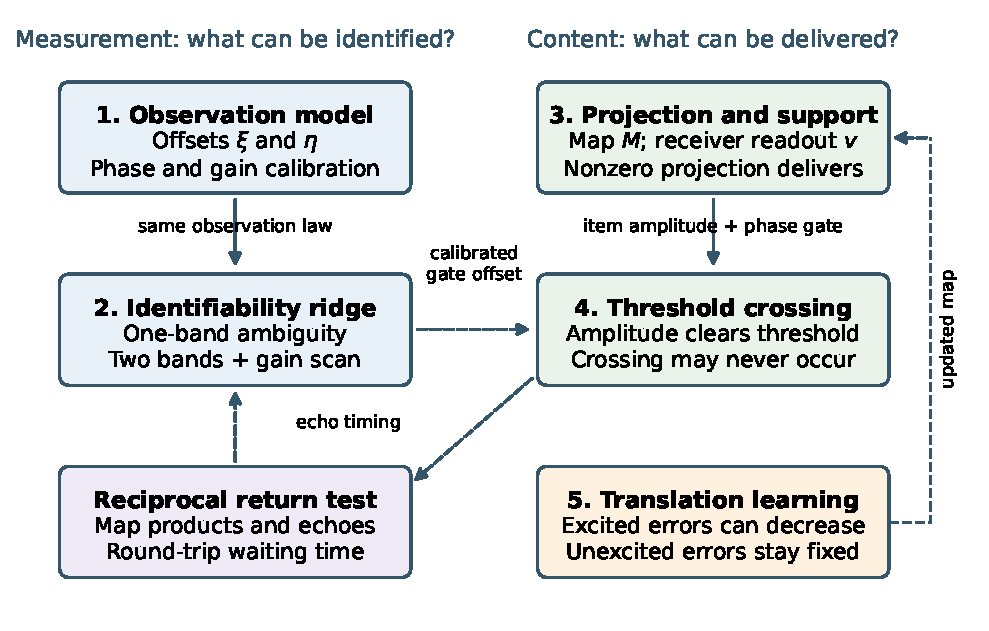
\includegraphics[width=.96\linewidth]{figure_roadmap.pdf}\caption{Conceptual roadmap linking observation, projection, completion, return, and learning.}\label{fig:roadmap}\end{figure}

The gate offset links observation to delivery. Reciprocal map products determine returning content; resolved echo timing supplies information outside the stationary ridge. Threshold crossing is separate from nonzero delivery. Learning changes the map between frozen calibration windows, while behavioral readout and bilinear integration remain explicitly specified extensions.

For an externally anchored item $z\in\R^d$, regional population features are $x_j=\Dj z$ and the target receiver representation is $\Di z$. The translation error is
\begin{equation}
\Bij=\Tij \Dj-\Di.\label{eq:dictionary}
\end{equation}
These maps are frozen from separate calibration data and evaluated on held-out items. Replacing $z$ by $Sz$ and $\Dj$ by $\Dj S^{-1}$, for invertible $S$, leaves predictions unchanged. Coordinates need external anchors; $\Tij$ is unconstrained outside the calibrated sender span.

\begin{proposition}[Exact translation on the modeled content space]\label{prop:translation}
A linear map $\Tij$ satisfying $\Tij \Dj=\Di$ exists if and only if $\Ker \Dj\subseteq\Ker \Di$.
\end{proposition}
\begin{proof}
We work in finite-dimensional real vector spaces. First suppose a linear $T_{ij}$ satisfies $T_{ij}D_j=D_i$. If $z\in\Ker D_j$, then $D_jz=0$, and hence $D_iz=T_{ij}D_jz=T_{ij}0=0$. Thus every sender-null item is receiver-null, giving $\Ker D_j\subseteq\Ker D_i$.

Conversely assume this kernel inclusion. On the subspace $S=\im D_j$, define $T_0(D_jz)=D_iz$. This definition must be independent of the chosen preimage. If $D_jz=D_jz'$, then $z-z'\in\Ker D_j\subseteq\Ker D_i$, so $D_iz=D_iz'$. Therefore $T_0$ is well defined. For $a,b\in\R$ and $u=D_jz$, $u'=D_jz'$, linearity of both encoding maps gives
\[
T_0(au+bu')=T_0(D_j(az+bz'))=D_i(az+bz')=aT_0u+bT_0u'.
\]
Choose a basis of $S$ and extend it to a basis of the sender feature space. Define $T_{ij}$ to equal $T_0$ on the first basis vectors and assign arbitrary values, for example zero, on the added vectors. Linear extension defines a map on the entire feature space. For every $z$, $D_jz\in S$, so $T_{ij}D_jz=T_0D_jz=D_iz$. This proves sufficiency. The arbitrary extension also explains why calibration on $S$ alone cannot identify $T_{ij}$ outside $S$.
\end{proof}
Thus a feature annihilated by $\Tij \Dj$ cannot be restored by opening that pathway's scalar timing gate. Alternative pathways or a different translation can carry it; this claim concerns a fixed pathway, not all routes in a brain.

\subsection{A retarded communication operator}\label{sec:delayed}
Let $h_{ij}$ be nonnegative, causal, and normalized, with finite first moment. During a frozen-map window, define the arrival error, the gate, and the transferred content by
\begin{equation}
\Delt_{ij}(t)=\wrap[\theta_j(t-\tauij)-\theta_i(t)-\alpha_{ij}],\label{eq:arrival}
\end{equation}
where $\wrap$ folds an angle into $(-\pi,\pi]$. The gate $g(\delta)=\exp\{\kappa(\cos\delta-1)\}$ satisfies $g(0)=1$ and $g(\pm\pi)=e^{-2\kappa}$. The finite parameter $\kappa\ge0$ controls concentration; larger $\kappa$ makes the receptive window narrower. The phases $\theta_j,\theta_i$ belong respectively to the sender and receiver, and $\tau_{ij}\ge0$ is conduction time.
\begin{equation}
g(\delta)=\exp\{\kappa(\cos\delta-1)\},\quad r_{ij}(t)=w_{ij}g(\Delt_{ij}(t)),\quad w_{ij}\ge0,\label{eq:gate}
\end{equation}
\begin{equation}
U_{ij}(t)=\int_0^\infty h_{ij}(s)r_{ij}(t-s)\Tij x_j(t-\tauij-s)\,ds.\label{eq:transfer}
\end{equation}
The gate is evaluated when content arrives, then the processing kernel integrates that arrival. This is an explicit modeling order, not a physiological identity. Distributed conduction delays could be represented by another kernel, but distinguishing two unconstrained convolutions requires additional measurements. Local recurrence and additional inputs may be added separately; they are not hidden inside $\alpha$.

For constant gain and one Fourier component, the transfer multiplier is $r\Tij e^{-i\Om\tauij}H_{ij}(\Om)$, with
\begin{equation}
H_{ij}(\Om)=\int h_{ij}(s)e^{-i\Om s}\,ds.\label{eq:kernel}
\end{equation}
Its phase adds processing information. If $H$ is unknown, an effective phase quantity can contain $\gamma+\Om\tau-\arg H(\Om)$, where $\gamma$ is a separate transfer phase under the chosen sign convention. It cannot identify three ingredients from one scalar. For small $\Om$, $-\arg H(\Om)/\Om$ tends to the kernel mean, but at finite frequency it need not equal that mean. This is why communication latency is not generally captured by one additional constant. In the theorem below the kernel is absent, known, or held fixed; it cannot silently enlarge the theorem's domain.

\begin{proposition}[Translation and temporal fidelity]\label{prop:bound}
Let $z(t)$ be Lipschitz with constant $L_z$, $r$ a constant nonnegative gain, $\mu_h=\int s h(s)\,ds$, and $U(t)=r\int h(s)TD_j z(t-\tau-s)\,ds$. Then
\begin{equation}
\|U(t)-\Di z(t)\|\le r\|B\|\|z(t)\|+|1-r|\|\Di z(t)\|
+r\|TD_j\|L_z(\tau+\mu_h).\label{eq:bound}
\end{equation}
\end{proposition}
\begin{proof}
Use the Euclidean vector norm and its induced operator norm, with $\tau\ge0$. Nonnegativity and normalization of $h$ imply $\int_0^\infty h(s)\,ds=1$. Add and subtract the undelayed translated vector to obtain the exact decomposition
\[
U(t)-D_iz(t)=r\int_0^\infty h(s)TD_j[z(t-\tau-s)-z(t)]\,ds
+rTD_jz(t)-D_iz(t).
\]
Since $B=TD_j-D_i$, the last two terms can be written as $rBz(t)+(r-1)D_iz(t)$. Their norm is at most $r\|B\|\|z(t)\|+|r-1|\|D_iz(t)\|$ by the triangle inequality.

For the integral term, the integral triangle inequality, the operator-norm bound, and Lipschitz continuity give
\begin{align*}
\left\|r\int_0^\infty h(s)TD_j[z(t-\tau-s)-z(t)]\,ds\right\|
&\le r\|TD_j\|\int_0^\infty h(s)L_z(\tau+s)\,ds\\
&=r\|TD_j\|L_z(\tau+\mu_h).
\end{align*}
The finite first moment makes this bound finite and justifies integrability of the time-displacement term. Summing the static and temporal bounds proves Eq.~\eqref{eq:bound}. No equality of current and delayed content was assumed.
\end{proof}
The last term compares with \emph{current} target content. Against the appropriately delayed target, temporal displacement is not itself a representation error. A correct dictionary map, sufficient gain, and timely arrival are distinct conditions. Supplementary material gives serial-path composition, marker channels, and ordering counterexamples.

\section{Conditional single-band non-identifiability}\label{sec:phase}
\citet{dowdall2023} showed that transmission delays can change coherence and Granger-causality estimates in bidirectional systems through interference, even when the underlying interactions are otherwise unchanged. Proposition~\ref{prop:orbit} addresses a different, narrower question: a calibrated stationary carrier-plus-gate likelihood has an exact compensating parameter direction $(-\Omega,-\Omega,1)$, while its phase-only submodel has rank one. This is an explicit identifiability result for the stated observation model, not a derivation of their bidirectional interference mechanism.

A real nonnegative gate changes amplitude; it does not rotate a complex carrier. We therefore distinguish the receptive center $\alpha$ in Eq.~\eqref{eq:arrival} from a transfer phase $\gamma$. In a stationary probe with simultaneous phase contrast $\psi$, write
\begin{equation}
y_{i\leftarrow j}(t)=b\,g(\psi-\alpha-\Omega\tau)e^{-i\gamma}x_j(t-\tau),\quad
x_j(t)=A_j e^{i(\Omega t+\phi_j)}.\label{eq:obs}
\end{equation}
Here $b>0$ is calibrated and any known processing phase is corrected separately. The sender--drive cross-spectrum has mean
\begin{equation}
S(\psi)=a\,g(\psi-\eta)e^{-i\xi},\qquad
\eta=\alpha+\Omega\tau,\quad\xi=\gamma+\Omega\tau,\quad a=b|A_j|^2>0.\label{eq:obsphase}
\end{equation}
The raw contrast $\psi=\wrap(\theta_j-\theta_i)$ is a probe covariate, not an observation equation for the unknown delay. Equating $\gamma$ and $\alpha$ would be an additional physiological assumption; the main analysis does not impose it.

\subsection{An explicit observation model}\label{sec:obsmodel}
At independent calibrated probe phases $\psi_n$, observe
\begin{equation}
\widehat S_n=S(\psi_n)+\varepsilon_n,\quad
\Re\varepsilon_n,\Im\varepsilon_n\stackrel{\mathrm{iid}}{\sim}N(0,s^2).
\label{eq:noisyS}
\end{equation}
Thus $\mathbb E|\varepsilon_n|^2=2s^2$ and
\begin{equation}
\ell=-\frac{1}{2s^2}\sum_n|\widehat S_n-S(\psi_n)|^2+\mathrm{const}.
\label{eq:loglik}
\end{equation}
For a mean vector $\mu$ its information is $\mathcal I_{kl}=s^{-2}\Re\sum_n(\partial_k\mu_n)^*\partial_l\mu_n$. A phase-only mean $a e^{-i(\gamma+\Omega\tau)}$ with fixed $a$ gives
\begin{equation}
\mathcal I_{\gamma,\tau}=\frac{Na^2}{s^2}
\begin{pmatrix}1&\Omega\\\Omega&\Omega^2\end{pmatrix}.\label{eq:Fisher}
\end{equation}
This matrix has rank one. The receptive center $\alpha$ is not identified by this phase-only observation.

\begin{proposition}[Single-band carrier and gate equivalence]\label{prop:orbit}
In Eqs.~\eqref{eq:obsphase}--\eqref{eq:noisyS}, every admissible shift
\[
(\gamma,\alpha,\tau)\longmapsto(\gamma+\Omega u,\alpha+\Omega u,\tau-u)
\]
leaves the complete conditional observation law unchanged. Its information has rank at most two and null direction $(-\Omega,-\Omega,1)$. Informative gain probes can identify $\eta$ and $\xi$ locally, but cannot identify all three underlying parameters in one band.
\end{proposition}
\begin{proof}
Write $p=(\gamma,\alpha,\tau)$ and $F(p)=(\xi,\eta)=(\gamma+\Omega\tau,\alpha+\Omega\tau)$. For $p_u=(\gamma+\Omega u,\alpha+\Omega u,\tau-u)$, direct substitution gives $F(p_u)=F(p)$. Consequently $S_n(p_u)=S_n(p)$ for every probe $\psi_n$. The noise covariance in Eq.~\eqref{eq:noisyS} is fixed, so the product Gaussian densities coincide at every possible observed vector. This proves equality of the complete conditional laws, not just equality of noiseless phases.

The Jacobian of $F$, in the stated parameter order, is
\[
J=\begin{pmatrix}1&0&\Omega\\0&1&\Omega\end{pmatrix}.
\]
It has two independent rows and satisfies $Jn=0$ for $n=(-\Omega,-\Omega,1)^\top$. By the likelihood chain rule, the parameter score is $J^\top$ times the offset score, so $\mathcal I_p=J^\top\mathcal I_FJ$. Therefore $\rank\mathcal I_p\le2$ and $\mathcal I_pn=0$.

The condition for attaining rank two can also be stated explicitly. At a probe, write $g_n=g(\psi_n-\eta)$ and $g_n'=g'(\psi_n-\eta)$. Then $\partial_\xi S_n=-ia g_ne^{-i\xi}$ and $\partial_\eta S_n=-a g_n'e^{-i\xi}$. Their real information cross-product is zero, because one derivative is a quadrature rotation of the other. Thus
\[
\mathcal I_F=\frac{a^2}{s^2}
\begin{pmatrix}\sum_n g_n^2&0\\0&\sum_n(g_n')^2\end{pmatrix}.
\]
The first diagonal entry is positive because $a>0$ and $g_n>0$. The second is positive precisely when at least one probe has $g_n'\ne0$. Under that informative-scan condition, $\mathcal I_F$ is positive definite and $\mathcal I_p$ has rank two. Its null space is exactly $\Ker J$, which is one-dimensional. Phase wrapping may add discrete aliases but does not alter this local null direction.
\end{proof}
Independent same-band observations improve precision along identified directions but do not change this null direction. Every statistic of an unchanged law is invariant in distribution. A prior can favor a point on the ridge without resolving likelihood identifiability. Phase wrapping also creates discrete aliases; all rank claims here are local on a calibrated branch.

\subsection{Observed phase scores are not arrival error}\label{sec:measures}
PLV-like consistency $|N^{-1}\sum_n e^{i\psi_n}|$ and PPC are invariant to constant rotation of their phase samples. They quantify concentration, not proximity to a receptive phase. Constant opposite-phase arrival can give consistency one while gain is $e^{-2\kappa}$.
For samples $S_n=a_n e^{i\psi_n}$, the absolute (unsigned) wPLI is
\begin{equation}
\widehat{\mathrm{wPLI}}=\frac{|\sum_n a_n\sin\psi_n|}{\sum_n a_n|\sin\psi_n|},\label{eq:wpli}
\end{equation}
when the denominator is nonzero \citep{vinck2011}. The triangle inequality bounds the numerator by the denominator, so this ratio lies in $[0,1]$. It is not generally rotation invariant. Along the full-law equivalence of Proposition~\ref{prop:orbit}, its distribution is unchanged because the entire observation law is unchanged. An arbitrary rotation of a cross-spectrum does not establish that equivalence.

\subsection{Measurements that can add a parameter direction}\label{sec:constructive}
With shared frequency-independent $\gamma$ and corrected processing phase, two unwrapped carrier offsets obey $\xi_k=\gamma+\Omega_k\tau$. Their design has rank two for distinct frequencies. A calibrated gain scan at the first frequency then supplies $\eta_1$ and $\alpha=\eta_1-\Omega_1\tau$. This combined design identifies all three parameters locally. Arbitrary frequency dependence of transfer phase removes this conclusion.
For independent offset errors of variance $s_\xi^2$ and $N$ trials in each of two bands,
\begin{equation}
\operatorname{Var}(\widehat\tau)=\frac{2s_\xi^2}{N(\Omega_2-\Omega_1)^2}.
\label{eq:delayvariance}
\end{equation}
Here the two-band design for $(\gamma,\tau)$ is $X_2=\bigl(\begin{smallmatrix}1&\Omega_1\\1&\Omega_2\end{smallmatrix}\bigr)$. Independent band means have variance $s_\xi^2/N$, and their difference cancels the common intercept: $\widehat\tau=(\bar\xi_2-\bar\xi_1)/(\Omega_2-\Omega_1)$. Adding the gain-center row yields the three-parameter design in Eq.~\eqref{eq:jointdesign}.

A known chirp $\theta(t)=\Omega_0t+at^2/2$, $a\ne0$, instead gives $Y_k=\gamma+\theta(t_k)-\theta(t_k-\tau)+e_k$ with slope $a\tau$ and variance $s_\xi^2/[a^2\sum_k(t_k-\bar t)^2]$. Excitation, calibrated phase, and unwrapping remain necessary. A known additive receiver reset changes the gain probe but supplies no independent delay constraint.
The simulations use 8 and 16 Hz, true delay 18 ms, 32 independent offsets per band, and phase SD 0.2 rad. Across 300 runs the delay SD is 1.006 ms, compared with the predicted 0.995 ms. A chirp with 128 times on $[0,1]$ s and slope 40 rad/s$^2$ has delay SD 1.511 ms. Sample count explains why this differs from earlier illustrative chirp numbers.

\subsection{From identification to delivery: an exact window}\label{sec:delivery}
For a fixed item $z$ and unit scalar readout $v$, put $M=TD_j$ and $A_v=|v^\top Mz|$. In an instantaneous amplitude model,
\begin{equation}
\mathcal C_v=A_vg(\delta),\quad \delta=\wrap(\psi-\eta),\quad
 g(\delta)=e^{\kappa(\cos\delta-1)}.\label{eq:delivered}
\end{equation}
At fixed $\psi$ and item, compensated changes of $\alpha,\tau$ preserve this amplitude. This says nothing about a transient content onset displaced by a changed conduction delay.
\begin{proposition}[Exact delivery window]\label{prop:delivery}
Let $A_v\ge0$, $\kappa>0$, and threshold $\theta>0$. If $A_v<\theta$, no phase passes. If $\theta\le A_ve^{-2\kappa}$, every phase passes. Otherwise, for $A_ve^{-2\kappa}<\theta\le A_v$, passage is equivalent to
\begin{equation}
|\delta|\le\arccos\left(1+\frac{\log(\theta/A_v)}{\kappa}\right).
\label{eq:tolerance}
\end{equation}
Also $g(\delta)\ge1-\kappa\delta^2/2$ for real $\delta$.
\end{proposition}
\begin{proof}
Assume $\kappa>0$, as required by the displayed inverse window. Let $d=|\wrap(\delta)|\in[0,\pi]$. On this interval, $\cos d$ decreases from 1 to $-1$, so the range of $g$ is $[e^{-2\kappa},1]$.

If $A_v<\theta$, then $A_vg(d)\le A_v<\theta$, including $A_v=0$. If $\theta\le A_ve^{-2\kappa}$, the lower gate bound gives $A_vg(d)\ge\theta$ for all $d$. These establish the first two cases, including their boundary inequalities.

In the remaining case $A_ve^{-2\kappa}<\theta\le A_v$, necessarily $A_v>0$. Division and logarithms preserve the inequality and yield
\[
A_vg(d)\ge\theta\ \Longleftrightarrow\
\cos d\ge1+\frac{\log(\theta/A_v)}{\kappa}.
\]
The right-hand side lies in $(-1,1]$. Since cosine is one-to-one and decreasing on $[0,\pi]$, this is equivalent to the window in Eq.~\eqref{eq:tolerance}. At $\theta=A_v$ its half-width is zero, so only perfect alignment passes.

Finally $1-\cos\delta\le\delta^2/2$ for every real $\delta$. Combining $e^{-x}\ge1-x$ for $x\ge0$ with $x=\kappa(1-\cos\delta)$ gives $g(\delta)\ge1-\kappa(1-\cos\delta)\ge1-\kappa\delta^2/2$. If $\kappa=0$, the gate is identically one and the threshold test is simply $A_v\ge\theta$; no inverse window is needed.
\end{proof}
The quadratic bound supplies a sufficient small-loss tolerance; it is not an exact necessary condition. At $\kappa=2$, gain at $\pi/4$ is 0.557; a 10\% loss target has exact half-width approximately 0.326 rad. For fixed positive amplitude weights $A_k$ and zero probe phases, a band sum $\mathcal C=\sum_k A_kg(\eta_k)$ has derivative $\mathcal C'(\tau)=-\kappa\sum_k A_k\Omega_k\sin(\eta_k)g(\eta_k)$. For example, offsets $\eta_1=\pi/2$, $\eta_2=-\pi/2$ and weights satisfying $A_1\Omega_1=A_2\Omega_2$ give a zero derivative even though each band contributes a nonzero derivative. A common delay therefore need not improve total delivery monotonically.

\paragraph{An identification design rather than a correlation test.}
The three effective measurements $(\xi_1,\xi_2,\eta_1)$ have parameter Jacobian
\begin{equation}
J=\begin{pmatrix}1&0&\Omega_1\\1&0&\Omega_2\\0&1&\Omega_1\end{pmatrix},
\qquad |\det J|=|\Omega_2-\Omega_1|.\label{eq:jointdesign}
\end{equation}
Consequently, a calibrated two-band carrier measurement and one informative gain scan resolve the local three-parameter ambiguity. This design connects the phase analysis to the delivery model: carrier phase estimates transfer, whereas the gain scan estimates reception. It fails when processing corrections or the shared transfer-phase assumption fail. These failures are experimentally distinguishable from a correct but imprecise fit.

\subsection{Why harmonics do not generically break the ridge}\label{sec:harmonics}
\begin{proposition}[Harmonic rank]\label{prop:harmonic}
For unwrapped carrier offsets $\xi_m=\gamma_m+m\Omega\tau$, $m=1,\ldots,M$, free $\gamma_m$ give design rank $M$ in $M+1$ parameters. Shared $\gamma_m=\gamma$ gives rank two for $M\ge2$ and $\Omega\ne0$. Harmonic-scaled $\gamma_m=m\gamma$ gives only $\xi_m=m(\gamma+\Omega\tau)$ and retains rank one.
\end{proposition}
\begin{proof}
Let $c=\Omega(1,\ldots,M)^\top$. With free transfer phases, the map from $(\gamma_1,\ldots,\gamma_M,\tau)$ to the offsets is multiplication by $[I_M\mid c]$. Its first $M$ columns already span $\R^M$, so its rank is $M$. A vector $(b,t)$ is in its null space exactly when $b+ct=0$, or $b=-ct$. Thus the null space consists of $t(-c,1)$ and has dimension one.

With shared transfer phase, the design is $[\mathbf1_M\mid c]$. Suppose $a\mathbf1_M+bc=0$. Comparing rows 1 and 2 gives $b\Omega=0$. If $M\ge2$ and $\Omega\ne0$, this implies $b=0$, and either row then implies $a=0$. The two columns are independent, so rank is two. If there is only one row or $\Omega=0$, that argument fails and rank cannot be two.

For harmonic-scaled phase, put $h=(1,\ldots,M)^\top$. The design becomes $[h\mid\Omega h]$, whose columns are proportional and whose first column is nonzero. Its rank is one; its null vector in $(\gamma,\tau)$ is $(\Omega,-1)$. A calibrated unwrapping branch or independent coarse latency bound is needed to exclude discrete aliases before applying these rank results. These computations concern unwrapped offsets under their respective parameter constraints. They do not resolve discrete phase aliases.
\end{proof}
These are assumptions on harmonic transfer phases, not a consequence of observing a nonsinusoidal waveform. Phase-slope methods likewise require response constraints \citep{nolte2008}.

\subsection{Common drive and the ridge}\label{sec:commondrive}
Observed analytic signals may be mixed as $x^{\rm obs}=x+c_jc$ and $y^{\rm obs}=y+c_ic$; their phases are arguments of these complex sums. Adding a complex carrier directly to a real angle is not a valid phase observation model.
\begin{proposition}[Parameter-independent observation channels]\label{prop:drive}
If the complete latent joint law is invariant under a parameter shift and the observation channel, including added common drive, is parameter independent, the observed law is also invariant.
\end{proposition}
\begin{proof}
Let $P_p$ denote the complete latent law at parameter $p$ and let $K(x,E)$ be the parameter-independent observation kernel: for latent state $x$, it is the probability that the measured observation falls in a measurable set $E$. The observed law is
\[
P_p^{\rm obs}(E)=\int K(x,E)\,P_p(dx).
\]
If a shift gives $P_{p'}=P_p$, integration against the same kernel gives $P_{p'}^{\rm obs}(E)=P_p^{\rm obs}(E)$ for every measurable $E$. Hence the observed probability measures coincide. Added common drive must be part of the invariant joint latent law or of this fixed kernel; equality of only the sender--receiver marginal need not suffice if the extra drive has parameter-dependent dependence on them. The result therefore preserves an existing equivalence under fixed observation channels without asserting equivalence for every common-drive generator.
\end{proof}
This conditional result does not claim that all common-drive models retain the same ridge. Additional parameter-dependent observations can add information. Unmodeled common drive can bias recovered phases even when it adds no justified identifying constraint.

\begin{figure}[htbp]\centering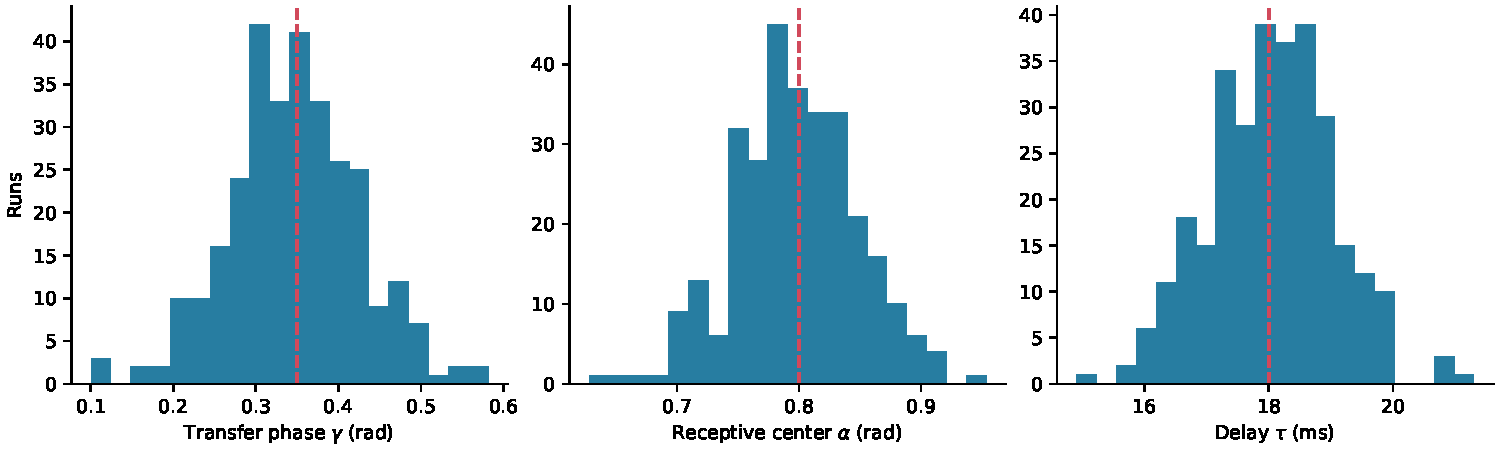
\includegraphics[width=.94\linewidth]{figure_joint.pdf}\caption{Synthetic joint recovery under the calibrated two-band and gain-scan design. The panels use the same $\gamma,\alpha,\tau$ notation as the revised source code. The 300 runs use truth $\gamma=0.35$ rad, $\alpha=0.8$ rad, and $\tau=18$ ms; correct specification and a calibrated unwrapped branch are assumed.}\label{fig:escape}\end{figure}

\section{Projected transfer, reciprocal feedback, and receiver readout}\label{sec:access}
An independently localized access circuit $A$ has incoming edges $\EA$. Define a route score $R=\sum_{(i,j)\in\EA}\lambda_{ij}r_{ij}$ with fixed nonnegative weights summing to one. This aggregate need not equal the gain of any particular content channel. Any report rule, decoder, threshold, and path aggregation must be frozen separately from confirmatory outcomes.

\subsection{Completion latency and report status}\label{sec:ridgeconstrains}
A stationary gain depends on $\eta$; its amplitude is invariant along the compensated shift in Proposition~\ref{prop:orbit}. An operational completion time inherits that invariance only when item amplitude trajectories, availability times, probe trajectories, thresholds, and relevant noise laws also stay fixed. Changing conduction can move a transient onset even if a carrier phase is compensated. Completion can be tested without identifying every parameter: testing an observable threshold law does not necessarily require breaking its parameter ridge. Distinguishing delay from receptive or transfer phase does require a transverse constraint.

\paragraph{Latency components and report status.}\label{sec:unreported-delay}
The generator contains conduction, processing kernels, and threshold waiting. It introduces no additional report-status latency parameter. This is a model specification, not proof that biology has no additional latency. For a constant offset and already available constant-amplitude one-way contribution, a threshold is either met immediately or never met. A changing offset can yield a finite hitting time; an absent projected vector cannot be repaired by scalar gain. With $\delta(t)=1.4-1.6t$ and half-width 0.5 rad, first entrance is 0.5625 s after the stated starting time. Reciprocal accumulation is a different possibility: Section~\ref{sec:reciprocal} derives a finite waiting time from delayed returns even when all gates remain constant.

\subsection{Projection sets the posting threshold}
The next results answer three successive questions. Can the pathway support the readout at all? Does the particular item produce a nonzero receiver contribution? Does that contribution reach the operational threshold? A positive answer to one question does not automatically answer the next.\label{sec:projection}
For $M=TD_j$, unit readout $v$, and item $z$, define
\begin{equation}
a_v(z,\delta)=|v^\top Mz|g(\delta).\label{eq:amplitude}
\end{equation}
The readout is structurally unsupported if $v\perp\im M$. It can receive some item if $v\notin(\im M)^\perp$. Membership $v\in\im M$ is not the criterion: a direction outside the image can still have nonzero projection onto it. Even a supported readout can have zero amplitude for a particular item.

\begin{lemma}[Structural support and item amplitude]\label{prop:projection}
The amplitude vanishes for every item and every phase if and only if $v^\top M=0$. For a fixed item, nonzero amplitude is equivalent to $v^\top Mz\ne0$, since $g(\delta)>0$ at every phase, including $\pi$.
\end{lemma}
\begin{proof}
Let $b=v^\top M$, a row acting on the item space. If $b=0$, then $bz=0$ for every item and $a_v(z,\delta)=0$ for every phase. Conversely, suppose $a_v(z,\delta)=0$ for every item and phase. Since $g(0)=1$, this implies $bz=0$ for every $z$. Applying it to each coordinate basis vector shows that every entry of $b$ is zero.

The equality $b=0$ is also equivalent to $v$ being orthogonal to $\im M$: each vector in that image has the form $Mz$, and its inner product with $v$ is $bz$. For a fixed item, the exponential gate is positive at every finite $\kappa$ and every phase. Thus $|bz|g(\delta)>0$ if and only if $bz\ne0$. This fixed-item statement is weaker than saying that every item is deliverable in a supported readout.
\end{proof}

\begin{theorem}[Nonzero projection establishes modeled interregional communication]\label{thm:inter}
Let $j$ and $i$ denote sender and receiver brain regions represented by the calibrated maps $D_j$ and $T_{ij}$. Put $M=T_{ij}D_j$. Consider an available item $z$, a unit receiver readout $v$, and the instantaneous isolated-path contribution
\begin{equation}
q_{i\leftarrow j,v}(z,\delta)=v^\top U_{ij}=g(\delta)v^\top Mz,\qquad
 g(\delta)=e^{\kappa(\cos\delta-1)},\quad 0\le\kappa<\infty.
\label{eq:communication}
\end{equation}
A fixed positive pathway weight is absorbed into $M$. Hold arrival phase, pathway map, and other receiver inputs fixed. Define communication through this pathway as a nonzero sender-dependent contribution to the receiver readout. Then:
\begin{enumerate}[label=(\roman*),leftmargin=*]
\item If the item's readout projection $v^\top Mz$ is nonzero, communication from $j$ to $i$ occurs at every arrival phase, including $\pi$. Its magnitude is $a_v=|q_{i\leftarrow j,v}|$, bounded by
\[
e^{-2\kappa}|v^\top Mz|\le a_v\le |v^\top Mz|.
\]
\item For a source-content perturbation $z\mapsto z+\epsilon d$ at fixed phase, the receiver contribution changes by
\begin{equation}
q(z+\epsilon d,\delta)-q(z,\delta)=\epsilon g(\delta)v^\top Md.
\label{eq:projectioncontrast}
\end{equation}
The contrast is exactly linear in the perturbation size $\epsilon$ at fixed phase. Thus a nonzero projected content contrast establishes a nonzero input--output effect in this model, rather than merely a similarity of regional representations.
\item The pathway supports communication in readout $v$ for some content contrast if and only if $v^\top M\ne0$, equivalently $v\notin(\im M)^\perp$. If $v^\top M=0$, this pathway cannot communicate into that readout through any scalar phase gate.
\end{enumerate}
\end{theorem}
\begin{proof}
For finite nonnegative $\kappa$, $-1\le\cos\delta\le1$ implies $-2\kappa\le\kappa(\cos\delta-1)\le0$. Exponentiating gives $0<e^{-2\kappa}\le g(\delta)\le1$. Multiplication by $|v^\top Mz|$ yields the magnitude bounds in (i). If that projection is nonzero, its product with a strictly positive gain is nonzero, including at $\delta=\pi$.

To prove (ii), hold the gate and map fixed and expand by linearity:
\begin{align*}
q(z+\epsilon d,\delta)-q(z,\delta)
&=g(\delta)v^\top M(z+\epsilon d)-g(\delta)v^\top Mz\\
&=\epsilon g(\delta)v^\top Md.
\end{align*}
For $\epsilon\ne0$ and $v^\top Md\ne0$, this is a nonzero receiver change. Other receiver contributions cancel from this contrast only under the stated matched-input assumption.

For (iii), if $b=v^\top M$ is nonzero, choose $d=b^\top$. Then $bd=bb^\top=\|b\|_2^2>0$. Taking any nonzero perturbation size gives a nonzero source-content effect by (ii). If $b=0$, both the item contribution and every content contrast vanish, independent of the phase. The equivalence to $v\notin(\im M)^\perp$ follows from the image characterization proved in Lemma~\ref{prop:projection}. Communication here is this specified source-dependent contribution; no report threshold or empirical pathway identification is used in the proof.
\end{proof}
The theorem establishes communication between the two regional variables within the specified transfer model. It does not establish from regional activity alone that this pathway exists in a brain. Empirical application requires independently calibrated maps and a source-content contrast with matched arrival phase and other inputs. Nonzero projection of a particular item establishes its modeled delivery; structural support alone establishes only the existence of a deliverable contrast. Opposite phase attenuates communication, rather than abolishing it.

\begin{corollary}[Communication and operational completion are distinct]\label{cor:completion}
For a fixed projected magnitude $A_v=|v^\top Mz|$ available at receiver time $t_0$, assume a continuous gain trajectory $t\mapsto g(\delta(t))$. Define thresholded posting and completion by
\begin{equation}
t_v^*=\inf\{t\ge t_0:A_vg(\delta(t))\ge\theta\},\quad\theta>0,\qquad
\inf\varnothing=\infty.\label{eq:completion}
\end{equation}
If $A_v<\theta$, completion is impossible even when Theorem~\ref{thm:inter} establishes nonzero communication. Otherwise the passing phases are exactly those of Proposition~\ref{prop:delivery}, and completion is their first attainment after $t_0$.
\end{corollary}
\begin{proof}
If $A_v<\theta$, the bound $g\le1$ implies that the set in Eq.~\eqref{eq:completion} is empty, so its infimum is $\infty$. Otherwise Proposition~\ref{prop:delivery} characterizes exactly when $A_vg(\delta(t))\ge\theta$. The set of passing times is consequently the set of times at which the gate trajectory enters that feasible phase region.

For the first-attainment claim, assume the gain trajectory $t\mapsto g(\delta(t))$ is continuous on $[t_0,\infty)$; a wrapped phase may jump at the branch cut while its gain remains continuous. The passing-time set $E$ is then closed relative to that interval, as the inverse image of $[\theta,\infty)$ under a continuous amplitude function. If $E$ is nonempty, its infimum $t^*$ is finite and at least $t_0$. Choose times $t_n\in E$ with $t^*\le t_n<t^*+1/n$. Then $t_n\to t^*$ and closedness implies $t^*\in E$. No earlier time belongs to $E$ by the definition of infimum. Hence the infimum is the first actual crossing. If $E$ is empty, completion is infinite, even when all instantaneous amplitudes are nonzero. Without gain continuity, an infimum need not be attained and should be called a crossing-time infimum rather than a first attained event.
\end{proof}
For nontrivial processing memory, apply the readout to Eq.~\eqref{eq:transfer}. Nonzero instantaneous projections can cancel under integration. A sufficient extension of Theorem~\ref{thm:inter}(i) is that $v^\top Mz(t-\tau-s)$ has one sign and magnitude at least $c>0$ throughout the processing support, with a normalized nonnegative kernel and positive fixed pathway weight $w$. Then $|v^\top U(t)|\ge wc e^{-2\kappa}>0$. This separates supported delivery from possible temporal cancellation.

\begin{proposition}[Communication certified under translation uncertainty]\label{prop:robustcommunication}
Let a calibrated estimate $\widehat M$ obey $\|M-\widehat M\|_2\le\epsilon_M$, with unit readout $v$ and fixed item $z$. Set
\[
\widehat A=|v^\top\widehat Mz|,\quad E=\epsilon_M\|z\|_2,
\quad A_- =\max(0,\widehat A-E),\quad A_+=\widehat A+E.
\]
For every phase, the true amplitude satisfies
\begin{equation}
A_-g(\delta)\le a_v\le A_+g(\delta).\label{eq:robustcommunication}
\end{equation}
If $\widehat A>E$, communication is nonzero for every admissible map and every phase. For threshold $\theta>0$, $A_-g(\delta)\ge\theta$ certifies posting, whereas $A_+g(\delta)<\theta$ certifies its absence. Intermediate cases are unresolved by the uncertainty bound.
\end{proposition}
\begin{proof}
Write $E_M=M-\widehat M$. The operator-norm assumption and $\|v\|_2=1$ give
\[
|v^\top E_Mz|\le\|v\|_2\|E_Mz\|_2\le\epsilon_M\|z\|_2=E.
\]
The triangle inequality gives $|v^\top Mz|\le|v^\top\widehat Mz|+E=\widehat A+E$. Its reverse form gives $|v^\top Mz|\ge\widehat A-E$. Combining the latter with nonnegativity of a magnitude gives $A_-\le|v^\top Mz|\le A_+$. Multiplication by the positive gate proves Eq.~\eqref{eq:robustcommunication}.

If $\widehat A>E$, then $A_->0$ and $a_v\ge A_-e^{-2\kappa}>0$ for every admissible map and phase. If $A_-g(\delta)\ge\theta$, every admissible amplitude is at least the threshold. If $A_+g(\delta)<\theta$, every admissible amplitude is strictly below it. These are sufficient certificates; when neither inequality holds, the bounds alone do not decide posting. A bound straddling the threshold does not assert that both outcomes are attainable by admissible maps, only that neither has been excluded by these inequalities.
\end{proof}
This result turns a near-zero fitted projection into a calibrated decision with uncertainty. A small estimated coefficient alone cannot establish structural absence. The bound is conditional on valid map uncertainty; it does not supply that uncertainty from the same confirmatory outcomes. If $A_->0$, the exact window of Proposition~\ref{prop:delivery} applied to $A_-$ gives phases with certified thresholded delivery. Applying it to $A_+$ gives an outer window of possible delivery. Their gap is an explicit target for better calibration.

\begin{proposition}[Two stages of communication]\label{prop:twostage}
A readout has either no structural support ($v^\top M=0$), or support for at least one item ($v^\top M\ne0$). For a supported fixed item, $a_v>0$ at every phase and gain continuously changes its magnitude from $A_ve^{-2\kappa}$ to $A_v$. Successful thresholded delivery is a separate event and may fail at every phase.
\end{proposition}
\begin{proof}
Let $b=v^\top M$. Either this row is zero or it is not; these cases are exhaustive and disjoint. In the zero case Lemma~\ref{prop:projection} shows that every item has zero amplitude. In the nonzero case choosing $z=b^\top$ gives $bz=\|b\|_2^2>0$, establishing support for at least one item.

Fix any item with $A_v=|bz|>0$. Theorem~\ref{thm:inter} gives $A_ve^{-2\kappa}\le a_v\le A_v$, so all phases have nonzero delivery. The gate is a continuous function on the phase circle and attains its minimum at opposite phase and maximum at zero; multiplication by $A_v$ gives the stated modulation range. Passing a positive threshold is governed instead by Corollary~\ref{cor:completion}. For example any threshold greater than $A_v$ is never passed, despite delivery at every phase. Thus support, delivery magnitude, and completion are separate statements.
\end{proof}
The projection stage establishes modeled sender-to-receiver delivery for a nonzero projected item and identifies which content contrasts can affect the receiver. Alignment specifies its amplitude. Thresholded posting and successful report require additional conditions. The gate has no exact closed phase at finite $\kappa$.

\paragraph{When communication becomes progressively less laggy.}
For two finite completion times, a measurable lag is $|t_p^*-t_c^*|$. Support alone imposes no sign on its change. For a monotone intervention $\delta_p(t)=\delta_0-qt$ starting above a feasible half-width $\vartheta$, $q>0$, first crossing is $(\delta_0-\vartheta)/q$ when this is after availability and before a wrap. Increasing $q$ reduces this crossing time. It reduces lag relative to a fixed earlier $t_c^*$ only while $t_p^*\ge t_c^*$. Beyond that point the absolute lag increases. An impossible threshold has infinite completion time, for which a two-path lag is not a finite measurement.

\begin{figure}[htbp]\centering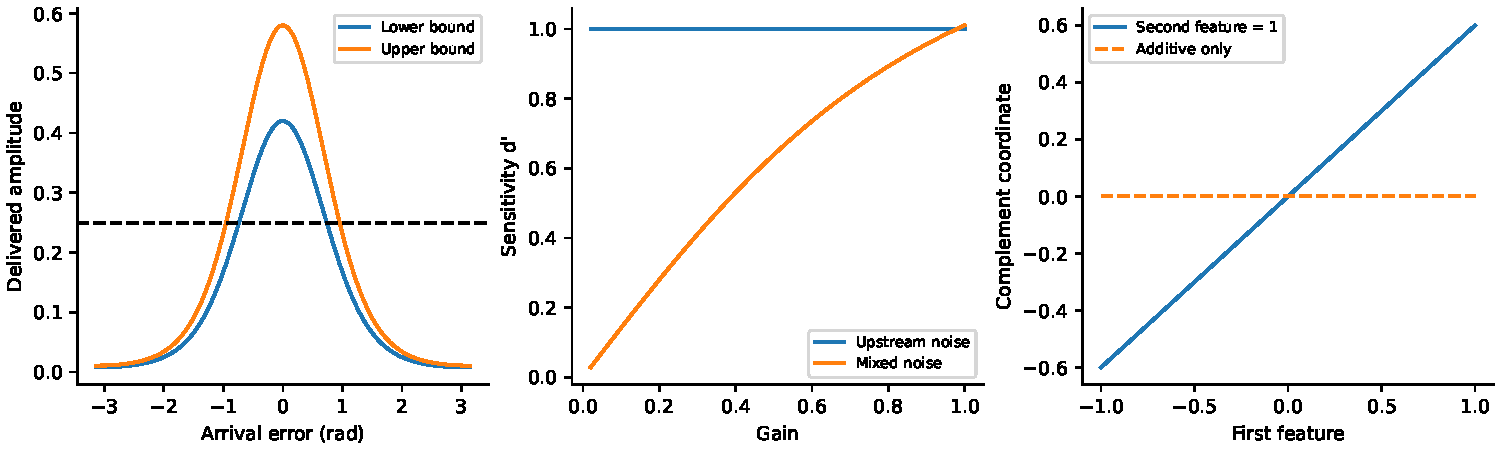
\includegraphics[width=.9\linewidth]{figure_delivery.pdf}\caption{Structural support, positive gain, and threshold feasibility are distinct. The gate remains positive at opposite phase. A nonzero projection can remain below threshold. First crossing depends on the specified phase trajectory.}\label{fig:projection}\end{figure}

\subsection{Reciprocal projection, feedback, and a recurrence waiting time}\label{sec:reciprocal}
The one-way projection result extends to a pair of calibrated populations. The new question is whether content sent in one direction can return in a direction that the first population reads. This requires a product of maps, not merely two individually nonzero maps. We derive both the carrier response and a time-domain threshold prediction from the same delayed feedback architecture. All maps and gains in this subsection are frozen; gain probes are externally calibrated rather than generated by the content feedback.

Let $P(t)\in\R^{n_P}$ and $Q(t)\in\R^{n_Q}$ be regional content features, where $n_P,n_Q$ are their feature dimensions, with independently timed external inputs $b_P,b_Q$. Absorb fixed positive gates and pathway weights into $L_{PQ}:\R^{n_Q}\to\R^{n_P}$ and $L_{QP}:\R^{n_P}\to\R^{n_Q}$. The first subscript denotes the receiver. These are the same operators as Section~\ref{sec:delayed}, closed into a reciprocal system, rather than a second unrelated model. For normalized causal processing kernels $h_f,h_b$, define
\begin{align}
(\mathcal L_f Q)(t)&=\int_0^\infty h_f(s)L_{PQ}Q(t-\tau_f-s)\,ds,\nonumber\\
(\mathcal L_b P)(t)&=\int_0^\infty h_b(s)L_{QP}P(t-\tau_b-s)\,ds.\label{eq:loop-operators}
\end{align}
The full loop is $P=b_P+\mathcal L_fQ$, $Q=b_Q+\mathcal L_bP$. On bounded signals, normalized nonnegative kernels give $\|\mathcal L_f\|\le\|L_{PQ}\|$ and $\|\mathcal L_b\|\le\|L_{QP}\|$. The product-norm condition below therefore makes the composite feedback operator a contraction, with solution
\[
P=(I-\mathcal L_f\mathcal L_b)^{-1}(b_P+\mathcal L_fb_Q)
=\sum_{k\ge0}(\mathcal L_f\mathcal L_b)^k(b_P+\mathcal L_fb_Q).
\]
This follows by substitution and convergence of the operator-norm geometric series. A return traverses both maps and both processing kernels. Their Fourier transforms multiply the corresponding carrier operators; time-domain echoes can consequently be dispersed rather than sharp jumps.

The discrete-delay equations used for the explicit latency result set each processing kernel to a unit point mass at zero. A point mass is not an integrable density under Section~\ref{sec:delayed}'s stated assumptions; it is an ideal limiting case. For example, the densities $h_\epsilon(s)=\epsilon^{-1}\mathbf{1}_{[0,\epsilon]}(s)$ satisfy those assumptions and concentrate at zero. For bounded continuous $Q$,
\begin{align*}
&\left\|\int h_\epsilon(s)L_{PQ}Q(t-\tau_f-s)\,ds-L_{PQ}Q(t-\tau_f)\right\|\\
&\qquad\le\|L_{PQ}\|\sup_{0\le s\le\epsilon}\|Q(t-\tau_f-s)-Q(t-\tau_f)\|\longrightarrow0.
\end{align*}
The analogous statement holds on the reverse edge. On bounded uniformly continuous signals this convergence is uniform in time; the common contraction bound then also gives convergence of the loop solutions through the resolvent identity. For step inputs, convergence is asserted away from discontinuities, not at the jump itself. Thus the sharp echo and integer-round-trip formula is a special instantaneous-processing limit; finite processing kernels require the convolutional first-passage calculation. In that limit specify
\begin{align}
P(t)&=b_P(t)+L_{PQ}Q(t-\tau_f),\nonumber\\
Q(t)&=b_Q(t)+L_{QP}P(t-\tau_b),\qquad \tau_f,\tau_b\ge0,\quad T_{\rm loop}=\tau_f+\tau_b>0.\label{eq:reciprocal}
\end{align}
The constant maps are translated receiver features, not raw anatomical connectivity. We use the sufficient stability condition $\|L_{PQ}\|\|L_{QP}\|<1$. General processing kernels would spread the echoes; their unknown phases and durations cannot be absorbed into an asserted conduction estimate.

\begin{theorem}[Reciprocal projected delivery and return support]\label{thm:reciprocal}
Assume Eq.~\eqref{eq:reciprocal}, zero prehistory, $b_P=0$, and a source step $b_Q(t)=d\,\mathbf{1}_{t\ge0}$. Write $A=L_{PQ}L_{QP}$. Then
\begin{equation}
P(t)=\sum_{k\ge0} A^k L_{PQ}d\,
\mathbf{1}_{t\ge\tau_f+kT_{\rm loop}}.\label{eq:echo}
\end{equation}
For a fixed readout $v$, the isolated $k$th increment is nonzero exactly when $v^\top A^kL_{PQ}d\ne0$. Direct projected delivery requires $v^\top L_{PQ}d\ne0$; an effective first return requires the additional condition $v^\top L_{PQ}L_{QP}L_{PQ}d\ne0$. The set of potentially delivered receiver features is contained in
\[
\mathcal S_d=\operatorname{span}\{L_{PQ}d,AL_{PQ}d,A^2L_{PQ}d,\ldots\}.
\]
A readout orthogonal to $\mathcal S_d$ never receives this item through the specified loop. At long times, $P(t)$ converges to $(I-A)^{-1}L_{PQ}d$.
\end{theorem}
\begin{proof}
Substitution of the second equation into the first gives
\[
P(t)=L_{PQ}d\,\mathbf{1}_{t\ge\tau_f}+A P(t-T_{\rm loop}).
\]
Before $\tau_f$ the forcing is zero and zero prehistory yields $P=0$. On $[\tau_f,\tau_f+T_{\rm loop})$ the delayed term still vanishes, so $P=L_{PQ}d$. Suppose the formula holds up to the $m$th interval. On the next interval, substituting its previous-interval value adds the term $A^{m+1}L_{PQ}d$ to the accumulated sum. Induction proves Eq.~\eqref{eq:echo}; for each finite time only finitely many terms are active because $T_{\rm loop}>0$. This also establishes the unique causal solution by the method of steps.

Subtracting the left limit from the value at $\tau_f+kT_{\rm loop}$ gives precisely $A^kL_{PQ}d$. Application of the linear functional $v^\top$ proves the increment criterion, including the direct and first-return cases. Every partial sum belongs to $\mathcal S_d$, so an orthogonal readout is identically zero. The bound $\|A\|\le\|L_{PQ}\|\|L_{QP}\|<1$ makes the infinite series absolutely convergent, since $\|A^kL_{PQ}d\|\le\|A\|^k\|L_{PQ}d\|$. Multiplying its partial sums by $I-A$ yields $L_{PQ}d-A^{m+1}L_{PQ}d$, whose last term tends to zero. Therefore the limit is $(I-A)^{-1}L_{PQ}d$. This argument concerns step responses of the stated stable model; it makes no claim that arbitrary matrix feedback increases every readout.
\end{proof}

\paragraph{Why two nonzero pathway maps are insufficient.} Take $L_{PQ}=\operatorname{diag}(1/2,0)$, $L_{QP}=\operatorname{diag}(0,1/2)$, and $d=v=e_1$. Both maps are nonzero, and the forward contribution is $1/2$, but $L_{QP}L_{PQ}d=0$: this item produces no return. Moreover, signed echo increments can cancel in a summed readout. Individually timed increments, rather than the nonzero status of each anatomical pathway, are the appropriate test of the product condition.

\begin{corollary}[An explicit recurrence contribution to completion latency]\label{cor:recurrence}
Suppose the delivered vector $p_0=L_{PQ}d$ lies in an invariant channel $Ap_0=\beta p_0$, with $a=v^\top p_0>0$ and $0\le\beta<1$. Define completion as the first time the signed readout reaches $\theta>0$. Then the readout on the $m$th interval is $a\sum_{k=0}^{m}\beta^k$. If $\theta\le a$, completion occurs at $\tau_f$. If $\beta=0$ and $\theta>a$, it never occurs. For $0<\beta<1$ and $a<\theta<a/(1-\beta)$,
\begin{align}
m_*&=\min\left\{m\in\{0,1,\ldots\}:\frac{a(1-\beta^{m+1})}{1-\beta}\ge\theta\right\},\nonumber\\
t_*&=\tau_f+m_*T_{\rm loop}.\label{eq:recurrence-latency}
\end{align}
If $\theta\ge a/(1-\beta)$ in this latter case, no finite completion occurs. A zero initial projected vector remains zero under the linear loop.
\end{corollary}
\begin{proof}
The eigenvector condition implies $A^kp_0=\beta^kp_0$ for every $k$ by induction. Apply $v^\top$ to Eq.~\eqref{eq:echo}. For $\beta=0$ the only nonzero increment is the first, proving the stated cases. For $0<\beta<1$ the partial sums increase strictly to $a/(1-\beta)$, so any threshold strictly between $a$ and that limit has a smallest finite crossing index. The series formula yields Eq.~\eqref{eq:recurrence-latency}. Each plateau begins with an attained right-continuous jump, so the first crossing is attained here without invoking the continuous-gain assumption of Corollary~\ref{cor:completion}. Every finite partial sum is strictly below its limit; equality with the limit therefore does not produce a finite crossing. If $p_0=0$, all powers of $A$ applied to it are zero. A zero direct scalar readout alone does not imply this last conclusion: feedback can rotate a nonzero vector into the readout at a later echo.
\end{proof}

With known source onset and resolved sharp increments, the first increment identifies $\tau_f$ and successive spacing identifies $T_{\rm loop}$, hence $\tau_b=T_{\rm loop}-\tau_f$. This constraint requires the instantaneous-processing limit and separation from measurement artifacts; finite unknown processing invalidates the direct conduction interpretation.

The additional term $m_*T_{\rm loop}$ is a derived accumulation waiting time. Projection and gates determine $a$ and $\beta$; conduction determines the spacing of successive opportunities. For $a=0.2$, $\beta=0.5$, $\tau_f=18$ ms, $\tau_b=12$ ms, and $\theta=0.34$, the readout steps through $0.2$, $0.3$, and $0.35$, crossing at 78 ms. This is 60 ms later than direct arrival. The same nonzero projection never reaches a threshold of $0.4$ at finite time. These examples replace the unsupported inference that nonzero projection ensures finite lag. The recurrence waiting time is distinct from the changing-phase waiting time in Section~\ref{sec:unreported-delay}; neither is an inferred universal duration of unreported processing.

\paragraph{Beyond an invariant channel.} Corollary~\ref{cor:recurrence} gives a closed scalar formula because all increments point in the same direction. General stable maps can rotate, cancel, or transiently amplify a readout. Their completion criterion is still explicit as a sequence of matrix partial sums, with a quantitative bound on the unresolved tail.

\begin{proposition}[General projected first passage and finite certification]\label{prop:generalpassage}
Under Theorem~\ref{thm:reciprocal}, put $p_0=L_{PQ}d$, let $v$ be a fixed readout, and set $q_A=\|A\|<1$. Define
\[
z_m=v^\top\sum_{k=0}^{m}A^kp_0,
\qquad z_\infty=v^\top(I-A)^{-1}p_0,
\qquad E_m=\frac{\|v\|\|p_0\|q_A^{m+1}}{1-q_A}.
\]
For a positive signed threshold $\theta$, the first attained event is $\tau_f+m_*T_{\rm loop}$, where $m_*=\min\{m\ge0:z_m\ge\theta\}$, or it never occurs if this set is empty. The tail satisfies $|z_\infty-z_m|\le E_m$. If $z_\infty>\theta$, completion is necessarily finite; any $m$ with $E_m<z_\infty-\theta$ is an upper bound on the crossing index. If all values through $M$ are below threshold and $z_\infty+E_M<\theta$, completion never occurs. Values $z_\infty\le\theta$ alone do not exclude an earlier transient crossing. For $n_P$ receiver coordinates, the readout is identically zero if and only if $v^\top A^kp_0=0$ for $k=0,\ldots,n_P-1$.
\end{proposition}
\begin{proof}
Equation~\eqref{eq:echo} is constant on each interval between consecutive return times, including its attained left endpoint. Applying $v^\top$ gives $z_m$ on the $m$th interval, proving the minimum-index rule without an invariance or positivity assumption. Absolute convergence yields
\[
|z_\infty-z_m|\le\|v\|\sum_{k=m+1}^{\infty}\|A\|^k\|p_0\|
=E_m.
\]
Since $E_m\to0$, if $z_\infty>\theta$ there is a finite $m$ with $z_m\ge z_\infty-E_m>\theta$. The first crossing is no later than this index. If $q_A=0$, the tail is zero and the first partial sum is already the limit. For every $m\ge M$, $E_m\le E_M$, so $z_m\le z_\infty+E_M<\theta$ certifies exclusion of all later crossings after the finite checked prefix. Equality in either bound does not provide the corresponding strict certification.

An identically zero readout has zero successive differences, so every $v^\top A^kp_0$ vanishes. Conversely, the Cayley--Hamilton identity expresses $A^{n_P}$ as a linear combination of lower powers. Multiplication by further powers and induction express all higher powers using $I,A,\ldots,A^{n_P-1}$. If the first $n_P$ scalar coefficients vanish, all subsequent ones vanish, and so does every partial sum. This proves the finite support test. None of these arguments requires $p_0$ to be an eigenvector.
\end{proof}

For example, take $A=\left(\begin{smallmatrix}0&0.5\\-0.5&0\end{smallmatrix}\right)$ and $p_0=v=e_1$. The first readout is 1, while its limit is 0.8; threshold 0.9 is crossed at direct arrival despite lying above the limit. Threshold 0.8, equal to the limit, is also crossed at direct arrival. Thus the scalar invariant-channel exclusion at equality is not general. With $p_0=e_1$, $v=e_2$, and $A=\left(\begin{smallmatrix}0&0\\0.5&0\end{smallmatrix}\right)$, the direct readout is zero and the first return is 0.5. Rotation into a readout can therefore create a later contribution even without scalar accumulation. For absolute-amplitude completion, replace $z_m\ge\theta$ by $|z_m|\ge\theta$; the same tail bound applies with $|z_\infty|$, while the signed example and minimum must be evaluated with the chosen rule.

\paragraph{Non-normal loops: contraction versus stability.} The Euclidean bound in Proposition~\ref{prop:generalpassage} can be conservative, but $\|A\|_2<1$ itself excludes growth of $\|A^kp_0\|_2$. A readout can nevertheless rise as the vector rotates. Genuine transient vector amplification requires a broader condition. The relevant extension is Schur stability, $\rho(A)<1$, where $\rho$ denotes the largest eigenvalue modulus. An $\varepsilon$-pseudospectrum describes sensitivity to perturbations and depends on $\varepsilon$; it is not a substitute for the norm bound used above.

\begin{proposition}[Stable non-normal return certification]\label{prop:stable-returns}
Retain the sharp-delay loop, zero prehistory, and step input of Theorem~\ref{thm:reciprocal}, but replace its product-norm condition by $\rho(A)<1$. The echo formula, finite Krylov support test, and first-passage rule still hold. Define
\[
G_A=\sum_{k=0}^{\infty}(A^k)^\top A^k,
\qquad q_G=\sqrt{1-1/\lambda_{\max}(G_A)}<1.
\]
This positive-definite matrix solves $G_A-A^\top G_AA=I$. With $\|p\|_G=\sqrt{p^\top G_Ap}$ and dual readout norm $\|v\|_{G^{-1}}=\sqrt{v^\top G_A^{-1}v}$, replace the Euclidean tail by
\begin{equation}
|z_\infty-z_m|\le
\|v\|_{G^{-1}}\|p_0\|_G\frac{q_G^{m+1}}{1-q_G}.
\label{eq:lyapunov-tail}
\end{equation}
All strict crossing/exclusion certificates in Proposition~\ref{prop:generalpassage} apply with this bound. Euclidean transient amplification is permitted.
\end{proposition}
\begin{proof}
Method-of-steps induction establishes the finite-time echo formula without any stability condition. For a finite matrix with $\rho(A)<1$, its Jordan form implies $\|A^k\|\le Cr^k$ for some $C<\infty$ and $\rho(A)<r<1$: each Jordan-block power is bounded by a finite polynomial in $k$ times its eigenvalue powers, and the polynomial is absorbed by the strictly larger exponential rate $r$. Nilpotent blocks vanish after finitely many powers. The series defining $G_A$ therefore converges absolutely. Its $k=0$ term is $I$, so $G_A\succeq I$ and is positive definite. Removing that term and shifting the convergent series proves the displayed Lyapunov identity.

For every vector $p$,
\[
\|Ap\|_G^2=\|p\|_G^2-\|p\|_2^2
\le(1-1/\lambda_{\max}(G_A))\|p\|_G^2.
\]
Thus the induced $G_A$ norm contracts by $q_G<1$. Cauchy--Schwarz after inserting $G_A^{1/2}$ and $G_A^{-1/2}$ gives $|v^\top p|\le\|v\|_{G^{-1}}\|p\|_G$. Applying this to the geometric tail yields Eq.~\eqref{eq:lyapunov-tail}. If $q_G=0$, the inequality forces $A=0$ and the tail is zero. The same convergent geometric-series identity gives $z_\infty=v^\top(I-A)^{-1}p_0$. Substitution of the new tail in the earlier strict certificates proves the claims. The finite support test uses Cayley--Hamilton alone and is unchanged. No normality, positivity, or scalar-channel assumption is needed.
\end{proof}

This is a standard Lyapunov construction applied to the paper's projected completion statistic. It extends the usable model class rather than introducing new stability mathematics. For
\[
A=\begin{pmatrix}0.65&1.2\\0&0.65\end{pmatrix},\quad
p_0=e_2,\quad v=e_1,
\]
$\rho(A)=0.65$ but $\|A\|_2>1$. The direct readout is zero; successive plateaus are $0$, $1.2$, $2.76$, $4.281$, and $5.5992$. Threshold $5$ is first reached on the fourth return, at 138 ms for the earlier 18/12 ms delays. The example's amplitudes are normalized illustrative output units. Supplementary Figure~S9 compares the actual tail with the certificate, and distinguishes Euclidean amplification from stability. Compute partial sums directly until a strict certificate is met; near equality, report unresolved status rather than treating a numerical tolerance as proof of crossing.


\paragraph{The same loop in the observation model.} At frequency $\Omega$, let the calibrated carrier operator on edge $e$ be
\[
K_e(\Omega,\psi_e)=g(\psi_e-\alpha_e-\Omega\tau_e)
e^{-i(\gamma_e+\Omega\tau_e)}M_e.
\]
Here $M_e$ is a fixed calibrated translation, and the transfer phase $\gamma_e$ remains distinct from receptive center $\alpha_e$. For the instantaneous real-map time-domain realization in Eq.~\eqref{eq:reciprocal}, $\gamma_e=0$; an unknown extra carrier transfer phase is an observation nuisance, not an additional delay in that step-response theorem. Known carrier processing factors can multiply $K_e$. Solving the two carrier equations gives
\begin{equation}
Y_P=(I-K_{PQ}K_{QP})^{-1}(B_P+K_{PQ}B_Q),\label{eq:loop-carrier}
\end{equation}
under $\|K_{PQ}\|\|K_{QP}\|<1$. This uses the same delayed map products as Eq.~\eqref{eq:echo}. It is a stationary carrier realization; a separately introduced frequency response must have a causal realization before it is used to predict broadband transients.

\begin{proposition}[Reciprocity alone does not resolve the single-band ridge]\label{prop:loop-ridge}
For fixed probes, maps, external input law, and parameter-independent observation noise, apply separately on either edge the admissible shift
\[
(\gamma_e,\alpha_e,\tau_e)\mapsto
(\gamma_e+\Omega u_e,\alpha_e+\Omega u_e,\tau_e-u_e).
\]
The complete stationary loop response and its observation law are unchanged. The six edge parameters consequently have at least two independent likelihood-null directions at one band. Time-resolved, independently anchored onsets and echoes need not inherit this invariance.
\end{proposition}
\begin{proof}
Both $\gamma_e+\Omega\tau_e$ and $\alpha_e+\Omega\tau_e$ remain unchanged on each edge. Therefore each complete $K_e$ remains unchanged, including its gain, and so do the product, inverse, and forcing in Eq.~\eqref{eq:loop-carrier}. Adding the fixed observation noise gives the same probability law. Differentiating the law along either edge shift gives zero score; the two shifts occupy disjoint parameter coordinates and are independent. Where regular Fisher information exists its rank is thus at most four. This is an upper bound, not a claim that every input or readout attains rank four. In contrast, Eq.~\eqref{eq:echo} contains $\tau_f$ in the first onset and $\tau_f+\tau_b$ in the spacing. Compensation of a phase at one frequency does not preserve these times. With known input onset, nonzero resolved increments, and known or absent processing, the first onset identifies $\tau_f$ and the spacing identifies the round-trip time, hence $\tau_b$. Missing or overlapping echoes remove that particular identifying argument.
\end{proof}

\paragraph{One model, two complementary tests.} Carrier calibration determines the gain and phase operators used to predict delivery; content perturbations and echo timing test those operators and provide transverse timing constraints that carrier observations alone lack. A matched reverse-path manipulation predicts a change in later echoes while the initial forward increment remains fixed. Learning changes the calibrated maps and hence the support and gain of the loop. The Gaussian readout below can be applied to a selected echo amplitude; the bilinear extension tests directions outside an independently calibrated additive response space. When feedback is present, that baseline must include its linear echo responses: feedback can itself rotate a feature into a previously silent readout. These are linked consequences and optional extensions of a common transfer architecture, rather than evidence that every assumption follows from the rank-one result.

\paragraph{Proposed prefrontal and interhemispheric application.} $P$ could be an independently localized prefrontal population and $Q$ a specified contralateral cortical population, with their report association measured separately. A hemisphere is not a single feature population, and prefrontal cortex is not assigned conscious status by anatomy. Prefrontal content decoding without volitional reports has been observed \citep{kapoor2022}; callosal delay estimates vary with axonal and pathway properties \citep{caminiti2013}. Neither study validates this loop model. Its test would calibrate both directed content maps, perturb each source independently, resolve the initial and returning increments, and assess Eq.~\eqref{eq:recurrence-latency} on held-out thresholds. The nonzero-projection criterion supports modeled communication between report-status populations, while the return-product criterion tests their reciprocal interaction. An additional physiological processing delay must be measured or modeled explicitly; it cannot be recovered from projection geometry alone.

\begin{figure}[htbp]\centering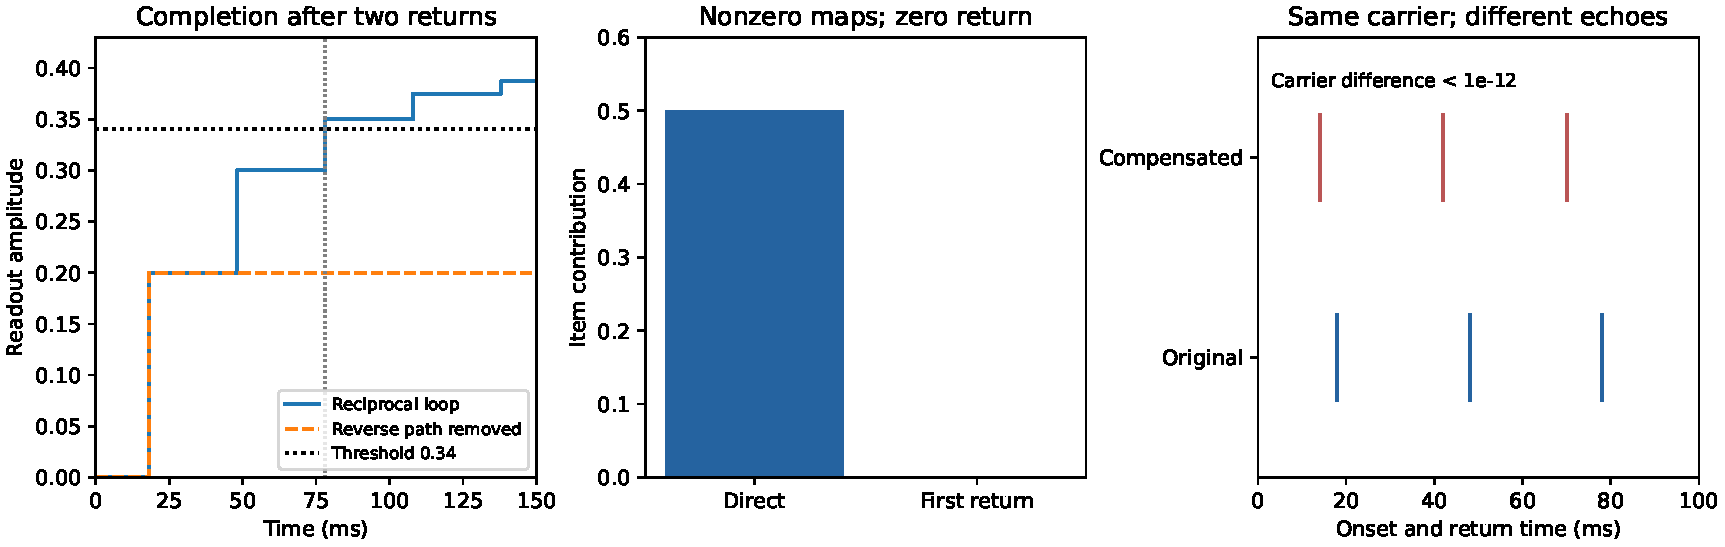
\includegraphics[width=.96\linewidth]{figure_reciprocal.pdf}\caption{Reproduced reciprocal-model checks. Left: positive aligned feedback reaches threshold after two returns; removing the reverse pathway preserves the first arrival but removes later increments. Middle: two nonzero maps can have a zero item-specific return product. Right: compensated edge parameters produce the same single-band carrier response but different directly anchored onset and echo times. Illustrative choices are $\tau_f=18$ ms, $\tau_b=12$ ms, direct amplitude $a=0.2$, return multiplier $\beta=0.5$, and threshold $\theta=0.34$.}\label{fig:reciprocal}\end{figure}

\subsection{Extension to nervous-system networks: supported routes and dispersed arrival}\label{sec:nervous-network}
The same architecture can represent a local, calibrated approximation to signaling between sensory, spinal, brainstem, cortical, or motor populations. Its variables are population features or small perturbations about a fixed operating state, not individual action potentials. The map describes a functional input--output projection; anatomical axonal projection alone does not identify that map. A constant-gain window is sufficient for the following extension, so oscillatory phase gating is optional. Chemical synapses, electrical coupling, refractory effects, and neuromodulatory state can require distinct kernels or nonlinear state equations outside this approximation.

The biological motivation is concrete. Auditory-brainstem experiments show that nodal and internodal geometry changes conduction timing \citep{ford2015}. Human PFC--M1 recordings support selective population-subspace transfer \citep{binish2026}. These observations motivate separate timing and projection quantities; neither establishes their particular combination here. In a sensorimotor return, muscle mechanics and sensory transduction also intervene. Those stages require calibrated operators and causal kernels rather than an additional unexplained ``communication delay.''

\paragraph{One network operator.} Let $N$ be the number of populations and $x_i(t)\in\R^{n_i}$ the perturbation features at population $i$. On each directed edge $j\to i$, let $L_{ij}:\R^{n_j}\to\R^{n_i}$ include its fixed nonnegative gate gain and its possibly signed translation map. Let $\tau_{ij}\ge\tau_{\min}>0$ be conduction time, and let $h_{ij}$ be a causal probability measure for residual processing. Densities recover Eq.~\eqref{eq:transfer}; a unit point mass recovers the ideal discrete-delay loop. With zero prehistory, define
\begin{equation}
x_i(t)=b_i(t)+\sum_{j:j\to i}\int_{[0,\infty)}L_{ij}x_j(t-\tau_{ij}-s)\,dh_{ij}(s).
\label{eq:network-transfer}
\end{equation}
Here $b_i$ is externally supplied content, not an unobserved recurrence term. The positive lower bound on edge conduction excludes instantaneous algebraic cycles. A useful sufficient bounded-signal stability condition is
\[
\rho_*:=\max_i\sum_{j:j\to i}\|L_{ij}\|<1,
\]
using the maximum of the population Euclidean norms. It is sufficient, not necessary, and stronger than some two-population stability conditions above.

For a directed walk $w=(j=i_0,i_1,\ldots,i_m=i)$, possibly visiting a population repeatedly, define its ordered translation, conduction sum, and processing measure by
\[
 L_w=L_{i_m i_{m-1}}\cdots L_{i_1i_0},\qquad
 \tau_w=\sum_{a=1}^m\tau_{i_ai_{a-1}},\qquad
 h_w=h_{i_mi_{m-1}}*\cdots*h_{i_1i_0}.
\]
For a source step $b_j(t)=d\mathbf1_{t\ge0}$, with content contrast $d\in\R^{n_j}$ and all other external inputs zero, set
\[
 F_w(t)=h_w([0,t-\tau_w])
\]
when $t\ge\tau_w$, and $F_w(t)=0$ otherwise. This cumulative processing response lies in $[0,1]$. A target readout $v\in\R^{n_i}$ is fixed independently of the tested trials.

\begin{theorem}[Supported-route arrival and threshold certificates]\label{thm:network}
For $i\ne j$, Eq.~\eqref{eq:network-transfer} has the unique causal solution
\begin{equation}
x_i(t)=\sum_{w:j\rightsquigarrow i}L_wd\,F_w(t),\qquad
 y_v(t)=v^\top x_i(t)=\sum_{w:j\rightsquigarrow i}c_wF_w(t),\quad c_w=v^\top L_wd.
\label{eq:walk-response}
\end{equation}
Only walks of length at most $\lfloor t/\tau_{\min}\rfloor$ can contribute at a finite time. Let $s_w=\inf\operatorname{supp}h_w$, and let
\[
 D_* =\inf_{w:c_w\ne0}(\tau_w+s_w),
\]
with $D_*=\infty$ when every coefficient is zero. Then:
\begin{enumerate}[label=(\roman*),leftmargin=*]
\item No target readout occurs before $D_*$. In particular, a faster anatomical route with $c_w=0$ cannot determine this item's readout onset. If every $c_w=0$, timing changes alone cannot create readout support while the maps remain fixed.
\item For instantaneous processing, aggregate walks with the same arrival time $D$ into $C_D=\sum_{w:\tau_w=D}c_w$. The first nonzero readout jump occurs at the smallest $D$ with $C_D\ne0$, if such a $D$ exists. A nonzero individual route is therefore not sufficient for an observed onset at its arrival time.
\item Define $B_v(t)=\sum_w|c_w|F_w(t)$. For an absolute readout threshold $\vartheta>0$, $B_v(t)<\vartheta$ certifies no completion at time $t$. For any selected walk $w_0$,
\[
 |y_v(t)|\ge |c_{w_0}|F_{w_0}(t)-\sum_{w\ne w_0}|c_w|F_w(t).
\]
If this lower bound is at least $\vartheta$, completion has occurred by $t$. These certificates permit signed maps, unequal delays, dispersion, and cancellation.
\end{enumerate}
Under $\rho_*<1$, the walk sum is also absolutely convergent uniformly for bounded source steps, and the bounded causal solution is unique on the entire time axis.
\end{theorem}
\begin{proof}
Write $\mathcal K$ for the edge-integral operator in Eq.~\eqref{eq:network-transfer}. Substituting $x=b+\mathcal Kx$ repeatedly gives
\[
 x=\sum_{m=0}^{M}\mathcal K^m b+\mathcal K^{M+1}x.
\]
Every application of $\mathcal K$ retards an argument by at least $\tau_{\min}$. Consequently the remainder vanishes at a fixed time $t$ as soon as $(M+1)\tau_{\min}>t$, using zero prehistory. The $m$th term expands over all length-$m$ directed walks. Ordered matrix multiplication gives $L_w$; integration of the scalar causal measures composes by convolution. Applied to a source step it yields $L_wd\,h_w([0,t-\tau_w])$. This proves Eq.~\eqref{eq:walk-response} and finite-time finiteness. The same substitution for the difference of two causal solutions makes that difference zero at each finite time, establishing uniqueness without a stability assumption.

A measure assigns no mass strictly below the infimum of its support. Thus every term with $c_w\ne0$ is zero for $t<\tau_w+s_w$; terms with zero coefficient vanish at every time. This proves (i), including the empty-set case. With point-mass processing, $F_w(t)=\mathbf1_{t\ge\tau_w}$. At any fixed arrival time the jump is therefore the finite sum $C_D$. If all earlier groups vanish, the readout before that time is zero, and its value after the jump is $C_D$. This proves (ii). The discrete arrival set is locally finite because of the positive edge-delay lower bound; hence any nonempty set of nonzero groups has a smallest member.

For (iii), apply the triangle inequality to the finite sum in Eq.~\eqref{eq:walk-response}; since $F_w\ge0$, the upper bound is exactly $B_v(t)$. Separate one term and apply the reverse triangle inequality to obtain the displayed lower bound. Meeting that sufficient lower bound implies the absolute readout meets threshold at $t$, whereas the upper-bound test excludes it at that time. It does not exclude an earlier transient crossing unless the upper-bound test holds throughout the earlier interval.

Finally, normalized measures and the block maximum norm imply $\|\mathcal K\|\le\rho_*$. The geometric series in $\mathcal K$ converges in operator norm when $\rho_*<1$. Expanding the series of edge norm products gives the scalar majorant $\|d\|\sum_{m\ge0}\rho_*^m$, which is finite. It bounds the summed norms of all vector walk contributions. Banach's contraction argument then supplies existence and uniqueness of the bounded solution. Stability is not asserted for networks failing this sufficient condition.
\end{proof}

\begin{lemma}[A less conservative weighted stability certificate]\label{lem:weighted-network}
Set $B_{ij}=\|L_{ij}\|$ on an edge and zero otherwise. If the spectral radius $\rho(B)<1$, Theorem~\ref{thm:network}'s uniform absolute convergence conclusion holds even when $\rho_*\ge1$. Equivalently, there are positive weights $q_i$ and $c<1$ such that $Bq\le cq$.
\end{lemma}
\begin{proof}
When $\rho(B)<1$, the matrix Neumann series converges and $q=(I-B)^{-1}\mathbf1=\sum_{m\ge0}B^m\mathbf1$ has every coordinate at least one. Thus $Bq=q-\mathbf1$ and $c=\max_i(1-1/q_i)<1$. In the weighted signal norm $\|x\|_q=\sup_{t,i}\|x_i(t)\|/q_i$, normalized processing measures give
\[
\|\mathcal Kx\|_q\le\max_i\frac{\sum_j B_{ij}q_j}{q_i}\|x\|_q\le c\|x\|_q.
\]
The geometric-series proof of Theorem~\ref{thm:network} now applies in this norm, also to the sum of the norms of walk contributions. Conversely, if $Bq\le cq$, the matrix $\operatorname{diag}(q)^{-1}B\operatorname{diag}(q)$ has row sums at most $c$. Its spectral radius, which equals $\rho(B)$, is at most $c<1$. This proves the equivalence and the certificate.
\end{proof}
For two scalar edge norms 2 and 0.4, the unweighted row bound is 2, whereas $\rho(B)=\sqrt{0.8}<1$; weights $(\sqrt5,1)$ recover the loop-product condition. Acyclic graphs have nilpotent $B$ and satisfy the weighted certificate regardless of individual finite edge gains. The criterion is exact for uniform absolute walk summability in the nonnegative scalar comparison network under unrestricted positive step forcing: its walk majorant is the matrix series $\sum_m B^m$, convergent exactly when $\rho(B)<1$. Signed maps and cancellations can yield bounded responses beyond this comparison condition, so it remains sufficient rather than necessary for the original network. Neither condition is needed for the finite-time causal construction.

\paragraph{How this extends the projection theorem.} Theorem~\ref{thm:inter} is the one-edge content contrast; Theorem~\ref{thm:reciprocal} selects alternating walks in a two-population loop; Theorem~\ref{thm:network} permits multiple intervening populations and competing routes. A direct null projection can coexist with an effective detour because the detour has a different map product. Conversely, a nonzero projection can remain below threshold or be canceled. The added latency is consequently item- and readout-specific. It is constrained by supported routes and their measured kernels, rather than a universal extra duration of unreported processing. With continuous processing densities, $D_*$ is a lower bound on arrival and need not be an attained nonzero event.

\paragraph{A test separating missing support from slow signaling.} Present two independently decoded source contrasts $d_1,d_2$ on the same anatomical route, freeze its maps, and estimate their arrival responses on held-out trials. The model permits $v^\top L_wd_1=0$ and $v^\top L_wd_2\ne0$ at the same conduction time. An additional supported detour can delay only the first contrast. Removing that detour should selectively remove its later response while preserving the second contrast's direct response. This requires an isolated intervention and a calibrated source contrast; ordinary cross-correlation cannot establish the route products.

\begin{proposition}[Dispersion and the conduction--processing ambiguity]\label{prop:dispersion}
Let an edge's residual causal processing time $S$ have finite mean $\mu$ and variance $\sigma_h^2$, and define $H(\Omega)=\mathbb E e^{-i\Omega S}$. At constant gain its temporal carrier factor is $e^{-i\Omega\tau}H(\Omega)$. Then
\begin{equation}
 |H(\Omega)-e^{-i\Omega\mu}|\le\tfrac12\Omega^2\sigma_h^2,
 \qquad |H(\Omega)|\ge\max\{0,1-\tfrac12\Omega^2\sigma_h^2\}.
\label{eq:dispersion-bound}
\end{equation}
Along a walk, convolution adds processing means and variances. Knowledge of the complete temporal response still does not generally separate conduction from an unconstrained processing kernel: if $S\ge u\ge0$ almost surely, replacing $(\tau,S)$ by $(\tau+u,S-u)$ leaves every temporal response unchanged.
\end{proposition}
\begin{proof}
Set $Z=S-\mu$, so $\mathbb EZ=0$ and $\mathbb EZ^2=\sigma_h^2$. For real $a$, the integral Taylor remainder of $e^{-ia}$ implies $|e^{-ia}-1+ia|\le a^2/2$. Therefore
\[
 |\mathbb E e^{-i\Omega Z}-1|
 =|\mathbb E(e^{-i\Omega Z}-1+i\Omega Z)|
 \le\tfrac12\Omega^2\mathbb EZ^2.
\]
Multiplication by $e^{-i\Omega\mu}$ proves the first bound. The reverse triangle inequality proves the second, with zero included because magnitude is nonnegative. A convolution of probability measures is the law of a sum of independent variables with those measures. Its mean is the sum of the means and its variance is the sum of the variances, proving the walk statement; dependence would require a different joint delay model. Finally, $\tau+u+(S-u)=\tau+S$ pointwise. The shifted variable remains causal by the assumed support gap. Thus its total impulse measure, Fourier transform, and responses to arbitrary inputs are identical. This last equivalence concerns constant-gain temporal operators; changing a time-varying gate requires a separate invariance argument.
\end{proof}

Dispersion can reduce carrier magnitude without removing structural support. For a causal uniform residual delay on $[\mu-a,\mu+a]$, $0<a\le\mu$, the exact magnitude is $|\sin(\Omega a)/(\Omega a)|$. Width is therefore an additional measurable quantity, not interchangeable with the mean delay or a null projection. Separating physiological travel time from synaptic integration needs a kernel constraint, two-site timing measurement, or another independent calibration even with broadband recordings.

\paragraph{Sharpness, other kernels, and independent timing.} The coefficient $1/2$ in Eq.~\eqref{eq:dispersion-bound} is asymptotically sharp. With $Z=S-\mu$ and finite second moment, dominated convergence applied to the second-order remainder gives $\mathbb E e^{-i\Omega Z}=1-\Omega^2\sigma_h^2/2+o(\Omega^2)$. For $\sigma_h^2>0$, the ratio of the first bound's two sides tends to one as $\Omega\to0$; a smaller universal coefficient is impossible. This does not assert equality at a nonzero frequency, and the lower magnitude bound becomes uninformative at sufficiently high frequency. For an exponential causal kernel of mean $\mu$, $H(\Omega)=(1+i\Omega\mu)^{-1}$ and $|H|=(1+\Omega^2\mu^2)^{-1/2}$; the same bound applies although this kernel is not uniform.

The ambiguity is broken by an independently known processing kernel, or by an imposed zero lower endpoint of its support together with resolved onset on an isolated, nonzero pathway: the lower endpoint of the total impulse measure is then $\tau$. An operational threshold crossing need not equal that endpoint. Two-site timing cancels downstream processing only when the two measurements share the same downstream stages and the measured interval isolates travel between the sites. Additional unknown stages restore ambiguity. Broadband measurements alone identify the total temporal operator, not its unconstrained decomposition. Supplement S20 gives non-uniform-kernel checks and numerical power calculations.

\paragraph{Faster travel need not mean earlier completion.} In an isolated scalar channel with unit source contrast, translation magnitude 0.5, $\psi=0$, $\kappa=2$, and a 40 Hz carrier, choose $\alpha=-\Omega(0.018)$ so that 18 ms conduction is aligned. Threshold 0.4 is met at the initial arrival in the instantaneous-processing step model. Shortening conduction to 13 ms with preference fixed produces $|\Delta|=0.4\pi$ and amplitude $0.5\exp[2(\cos(0.4\pi)-1)]\approx0.126$, which never reaches that threshold without another input or alignment change. Compensating preference by the opposite phase shift restores amplitude 0.5 and completion at 13 ms. This is a conditional content-by-timing prediction, not a claim that changing myelin affects only conduction. It links the identifiability calibration directly to the network's completion test: measured timing and calibrated gain must jointly predict the response.

\begin{figure}[htbp]\centering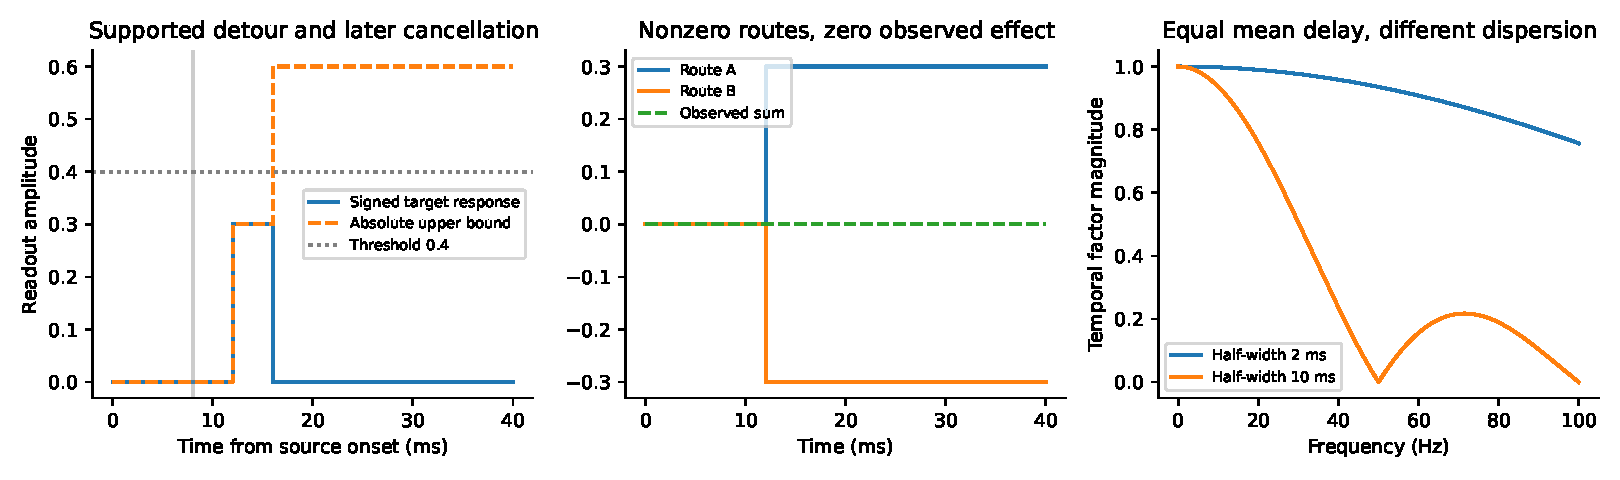
\includegraphics[width=.98\linewidth]{figure_nervous_network.pdf}\caption{Synthetic nervous-network illustrations; the separate randomized verification uses 100 networks with four populations and two features per population. Left: a fast 8 ms route has zero item projection, while a supported detour arrives at 12 ms. An opposing 16 ms route cancels the sustained readout. Middle: equal and opposite simultaneous route contributions cancel completely. Right: normalized causal uniform processing kernels with the same 15 ms mean and half-widths 2 and 10 ms retain different carrier magnitudes. These are model consequences, not measured physiological delays.}\label{fig:nervous-network}\end{figure}


\subsection{The sensitivity prediction}\label{sec:sdt}
Two complementary questions now require different models. A signal-detection readout connects delivered content to behavioral sensitivity. A bilinear pathway model, introduced below, asks whether joint inputs generate receiver directions that additive transfer cannot reach. The sensitivity result does not imply the interaction-rank result, and the interaction-rank result does not by itself imply a behavioral benefit.

An auxiliary Gaussian signal-detection model specifies how delivery affects a behavioral measure. For stimulus class $s\in\{-1,1\}$,
\begin{align}
X\mid s&=r\left(shC/2+\underbrace{\varepsilon_u}_{\text{upstream noise}}\right)
+\underbrace{\varepsilon_d}_{\text{downstream noise}},\notag\\
d'(r,C)&=\frac{rhC}{\sqrt{r^2\sigma_u^2+\sigma_d^2}}.\label{eq:sensitivity}
\end{align}
where $C\ge0$ is content magnitude, $r\ge0$ is channel gain, $h\ge0$ is calibrated content efficacy, and the independent zero-mean Gaussian noises $\varepsilon_u,\varepsilon_d$ have variances $\sigma_u^2,\sigma_d^2$.
\begin{corollary}[Conditional content-by-gain prediction]\label{cor:contentrouting}
Under Eq.~\eqref{eq:sensitivity}, for $hC>0$ and $\sigma_d>0$,
\[
\frac{\partial d'}{\partial r}=\frac{hC\sigma_d^2}{(r^2\sigma_u^2+\sigma_d^2)^{3/2}}>0,
\quad
\frac{\partial^2d'}{\partial C\partial r}=\frac{h\sigma_d^2}{(r^2\sigma_u^2+\sigma_d^2)^{3/2}}>0.
\]
For a null efficacy $h=0$ both are zero. With only upstream noise of positive variance, sensitivity is constant for $r>0$.
\end{corollary}
\begin{proof}
Let the two Gaussian noises be independent of one another and of class $s$, with zero means and variances $\sigma_u^2$ and $\sigma_d^2$. At fixed $r$, $X\mid s$ is Gaussian with mean $rshC/2$ and common variance $V(r)=r^2\sigma_u^2+\sigma_d^2$. The difference of the two class means is $rhC$. Dividing it by the common standard deviation gives Eq.~\eqref{eq:sensitivity} whenever $V(r)>0$.

Differentiate $rhC V(r)^{-1/2}$ using the product and chain rules:
\begin{align*}
\partial_r d'&=hC V^{-1/2}-r^2hC\sigma_u^2V^{-3/2}\\
&=hC[V-r^2\sigma_u^2]V^{-3/2}
=hC\sigma_d^2V^{-3/2}.
\end{align*}
Because $V$ is independent of content magnitude $C$, differentiating this expression with respect to $C$ gives $h\sigma_d^2V^{-3/2}$. With positive downstream noise, the denominator is positive even at $r=0$, and the claimed signs follow. If $h=0$, both derivatives are zero.

If $\sigma_d=0$ but $\sigma_u>0$, then for $r>0$, $d'=rhC/(r\sigma_u)=hC/\sigma_u$, independent of gain. At $r=0$ this pure-upstream model is degenerate; the displayed ratio is undefined rather than a positive-gain sensitivity result. These conclusions use the Gaussian readout and fixed noise variances, not just monotonicity of delivered amplitude.
\end{proof}
This prediction requires the readout and noise assumptions. Geometry alone, or monotonicity alone, does not entail a positive global regression coefficient $\beta_{CR}$. A route aggregate $R$ must be calibrated to the tested gain before substitution. Saturation can reverse a mixed derivative despite increasing sensitivity in each input. A nonsignificant interaction does not reject structural projection; a well-powered interval excluding a preregistered meaningful effect can reject the complete specified behavioral model.

The next model concerns receiver geometry before a behavioral readout is chosen. Its output can be used by a separately specified decision model, but substituting it into the scalar Gaussian readout would require new distribution and noise assumptions. Let translated pathway outputs $U,V$ share receiver coordinates. A fixed bilinear map $\Bmap$ into the receiver feature space, an integrable scalar memory kernel $k(s,q)$, and a real interaction coefficient $\chi$ define
\begin{equation}
I(t)=\chi\int_0^\infty\!\int_0^\infty k(s,q)\Bmap(U(t-s),V(t-q))\,ds\,dq,
\quad y(t)=U(t)+V(t)+I(t)+\epsilon(t).\label{eq:mixed}
\end{equation}
Here $\epsilon(t)$ is additive observation error with a fixed conditional mean across the contrasted conditions. For example, $k(s,q)=k_1(s)k_2(q)$ is a scalar separable memory. Conduction is already included in $U,V$. This is a constrained second-order input--output model \citep{korenberg1996}. A projection $Q$ annihilating $\im M_1+\im M_2$ removes the additive terms, leaving $Qy=QI+Q\epsilon$. A new coordinate requires a nonzero projected bilinear output; it does not arise automatically from alignment. Off-phase gates can still produce a nonzero interaction, and memory can combine inputs from different times.
The pair $(\Bmap,k)$ is ambiguous at least under $\Bmap\mapsto c\Bmap$, $k\mapsto k/c$, $c\ne0$. Fixing a normalization or independently measuring a component is necessary. An arbitrary invertible output transformation is not observationally equivalent without compensating the measurement map.

\begin{proposition}[Cross-path factorial contrast]\label{prop:contrast}
Hold content, kernels, maps, and noise mean fixed. Independently scale the two inputs by $a,b\in\{H,L\}$. Then
\begin{equation}
y_{HH}-y_{HL}-y_{LH}+y_{LL}
=\chi(H-L)^2\int\!\int k(s,q)\Bmap(U(t-s),V(t-q))\,ds\,dq.\label{eq:contrast}
\end{equation}
\end{proposition}
\begin{proof}
Denote the unscaled interaction integral by $J(t)=\int\!\int k(s,q)\Bmap(U(t-s),V(t-q))\,ds\,dq$, assumed to exist. For constant scales $a,b$, bilinearity gives $\Bmap(aU,bV)=ab\Bmap(U,V)$ at every integration point. Thus the interaction integral is $abJ(t)$. With fixed mean noise $m(t)$, each condition has mean $y_{ab}(t)=aU(t)+bV(t)+\chi abJ(t)+m(t)$.

The alternating four-condition sum gives coefficients $H-H-L+L=0$ on $U$, $H-L-H+L=0$ on $V$, and $1-1-1+1=0$ on the fixed noise mean. Its interaction coefficient is $H^2-HL-LH+L^2=(H-L)^2$. This proves Eq.~\eqref{eq:contrast}. The same cancellation removes any separable terms $f(aU)+j(bV)$, since each is added once and subtracted once for each scale. A joint nonlinear term need not factor or cancel, so the identity does not localize the anatomical interaction.
\end{proof}
Separable univariate nonlinearities also cancel. A joint nonlinear downstream readout can produce the same contrast. The test distinguishes cross-path dependence from separable alternatives under matched inputs, not its anatomical origin or experiential meaning.

\paragraph{Why rank is the relevant quantity.} A cross-path contrast can be nonzero while remaining in directions already carried by either pathway. To test whether an interaction adds a distinct receiver direction, first remove the additive space and then count independent remaining directions. The following proof establishes exactly what that count measures.

\begin{proposition}[How much new receiver content an interaction can add]\label{prop:innovation}
Let two independently controllable translated spaces be $S_1=\im M_1$ and $S_2=\im M_2$ in $\R^n$, with dimensions $r_1,r_2$. Put $S=S_1+S_2$, $A=[M_1\ M_2]$, and let $Q$ project orthogonally onto $S^\perp$. For orthonormal bases $p_a$ of $S_1$ and $q_b$ of $S_2$, form the columns $C_B=[\Bmap(p_a,q_b)]_{a,b}$. With a fixed nonzero coefficient $\chi$ and unrestricted independent inputs, the linear span of possible outputs $u+v+\chi\Bmap(u,v)$ is $S+\im C_B$. The number of added independent receiver directions is
\begin{equation}
d_B=\rank[A\ C_B]-\rank A=\rank(QC_B)
\le\min(n-\dim S,r_1r_2).\label{eq:innovationrank}
\end{equation}
Complement factorial contrasts spanning all independent basis pairs recover the effective added span, under the fixed-input conditions of Proposition~\ref{prop:contrast}.
\end{proposition}
\begin{proof}
Let $L$ be the linear span of all possible outputs and let $W=S+\im C_B$. Express $u=\sum_a x_ap_a$ and $v=\sum_b y_bq_b$. Bilinearity gives $\Bmap(u,v)=\sum_{a,b}x_ay_b\Bmap(p_a,q_b)$, so every output lies in $W$ and $L\subseteq W$.

For the reverse inclusion, unrestricted independent inputs include $(u,0)$, $(0,v)$, and $(0,0)$. Their outputs are $u$, $v$, and zero, so $S\subseteq L$. Subtract the two single-input outputs from a joint output:
\[
y(u,v)-y(u,0)-y(0,v)=\chi\Bmap(u,v).
\]
This difference belongs to $L$, which is a linear space. Since $\chi\ne0$, each basis-product vector $\Bmap(p_a,q_b)$ belongs to $L$. Therefore $\im C_B\subseteq L$ and $W\subseteq L$, proving equality.

The columns of $[A\ C_B]$ span $W$, while those of $A$ span $S$. The restriction of $Q$ to $W$ has kernel $S$: a vector in $W$ is killed exactly when it lies in $S$. Its image is $\im(QC_B)$, because $Q$ kills $A$ and every remaining column is a projected product. Rank--nullity on $W$ therefore yields $\dim W-\dim S=\rank(QC_B)$, establishing both rank equalities. The projected products lie in the $(n-\dim S)$-dimensional complement and are spanned by $r_1r_2$ columns, proving the upper bound.

Finally, Proposition~\ref{prop:contrast} applied to each basis pair and followed by $Q$ gives $\chi(H-L)^2Q\Bmap(p_a,q_b)$. For $H\ne L$ this is a common nonzero scalar multiple of each projected product. Their span equals $\im(QC_B)$, regardless of the value of that nonzero scalar. This identifies an effective output span across conditions, not each vector's attainability in a single condition or the location of the nonlinearity.
\end{proof}
The rank statement is unchanged if other bases are used: changing either basis multiplies the basis-product representation by invertible transformations and preserves its column span. The result concerns a linear span across input pairs and their contrasts. A single stimulus pair may excite only one direction; not every vector in that span need be attainable in one trial. It gives a concrete prediction beyond detecting a nonzero interaction: calibrated contrasts can test whether content occupies receiver directions that neither additive pathway reaches. A joint nonlinear receiver readout remains an alternative anatomical explanation. Restricted content co-variation, uncalibrated measurement nonlinearities, and memory cancellation must be excluded before interpreting the effective rank.

\paragraph{From added rank to measurable sensitivity.} Proposition~\ref{prop:innovation} identifies available receiver directions, not their behavioral use. The following readout model supplies the missing link. It connects the projected factorial contrast to discriminability, and specifies when added rank is behaviorally silent.

\begin{corollary}[Interaction innovation and Gaussian discriminability]\label{cor:rank-sensitivity}
Let the additive space $S$ and product matrix $C_B$ be those of Proposition~\ref{prop:innovation}. At a frozen analysis time, assume a receiver decision vector
\[
Y\mid s\sim N(s\mu/2,\Sigma),\quad s\in\{-1,1\},\qquad
\mu=\mu_S+\lambda b,
\]
where $\mu_S\in S$ is the additive class-mean contrast, $b\in\im C_B$ is a class-dependent bilinear contrast, $\Sigma$ is a fixed positive-definite noise covariance, and $\lambda=\chi a_1a_2$ for calibrated nonnegative pathway gains $a_1,a_2$. Write $W=\Sigma^{-1/2}$, and let $Q_\Sigma$ project orthogonally onto $(WS)^\perp$ in noise-whitened coordinates. The optimal linear discriminability in the innovation subspace is
\begin{equation}
d'_{\rm new}=|\lambda|\|Q_\Sigma Wb\|.\label{eq:innovation-sensitivity}
\end{equation}
The dimension of available noise-whitened innovation is $\rank(Q_\Sigma WC_B)=d_B$. Thus $d_B>0$ permits a positive interaction-only sensitivity for some class-dependent basis contrast, but does not guarantee it for a particular task or readout. Full optimal discriminability satisfies
\[
(d'_{\rm opt})^2=\|(I-Q_\Sigma)W\mu\|^2
+\lambda^2\|Q_\Sigma Wb\|^2.
\]
For fixed nonzero $Q_\Sigma Wb$, increasing $|\lambda|$ increases innovation-only discriminability. This conclusion requires fixed covariance and a decision rule that reads that subspace.
\end{corollary}
\begin{proof}
Whitening gives $WY\mid s\sim N(sW\mu/2,I)$. Projection removes the additive contrast, because $Q_\Sigma W\mu_S=0$. In an orthonormal basis of the range of $Q_\Sigma$, the projected noise covariance is identity and its class-mean difference is $\lambda Q_\Sigma Wb$. For a linear readout vector $w$ in that range, discriminability is $|w^\top\lambda Q_\Sigma Wb|/\|w\|$. Cauchy--Schwarz bounds this by the norm of the mean difference, with equality for a readout parallel to it when it is nonzero. If the difference is zero, every such readout has zero discriminability. This proves Eq.~\eqref{eq:innovation-sensitivity}.

Invertibility of $W$ preserves the dimensions of $S$ and $S+\im C_B$. Applying the quotient-rank argument of Proposition~\ref{prop:innovation} after whitening therefore gives $\rank(Q_\Sigma WC_B)=\dim(S+\im C_B)-\dim S=d_B$. The decomposition of $W\mu$ into its orthogonal additive and complement parts gives the squared full discriminability by Pythagoras. The complement part equals $\lambda Q_\Sigma Wb$, proving the displayed formula. Its norm is linear in $|\lambda|$ under the fixed covariance assumption. The additive part can also change with $\lambda$, so this result does not assert that total discriminability must exceed an additive-only baseline.
\end{proof}

This connects the geometric and behavioral tests in one design: estimate a complement factorial contrast on held-out trials, establish that it changes between stimulus classes, estimate its noise covariance independently, then test the sensitivity predicted by Eq.~\eqref{eq:innovation-sensitivity}. A positive added rank can carry only a class-independent interaction and contribute no discriminability. For example, flipping both inputs $(u,v)\mapsto(-u,-v)$ leaves $\Bmap(u,v)$ unchanged, so a class contrast based only on that paired reversal has $b=0$ despite possible nonzero interaction rank. Likewise, a fixed readout orthogonal to the innovation is insensitive to it. Gain-dependent upstream noise can cancel the benefit, as in Eq.~\eqref{eq:sensitivity}; the present fixed-$\Sigma$ corollary isolates the condition under which rank becomes a behavioral opportunity. This is a bridge through an explicit decision model, not a claim that rank alone entails awareness or a positive regression interaction.

\paragraph{Readout scope.} The discriminability formula assumes a fixed analysis time, fixed positive-definite covariance, and access to the optimal linear readout. A fixed biological decoder need not realize it. Nonlinear decisions or condition-dependent noise require a separate likelihood and sensitivity analysis; the geometric rank remains well defined but need not confer behavioral benefit.


\subsection{A slower trace is a separate postulate}\label{sec:plastic}
At presentation $n=0,1,\ldots$, let $T_n$ be the current linear translation, $u_n$ the sender teaching feature, $v_n$ its receiver target, $r_n\ge0$ its calibrated gain, and $\varepsilon>0$ the learning step size. With independently assigned learning-opportunity flag $\ell_n\in\{0,1\}$, retain
\begin{equation}
T_{n+1}=T_n+\varepsilon\ell_n r_n(v_n-T_nu_n)u_n^\top.\label{eq:plastic}
\end{equation}
For a repeated pair the residual contracts when $0<\varepsilon\ell_nr_n\|u_n\|^2<2$. If $\ell_n=0$, the map is frozen by construction. An access--trace split in this generator does not validate a synaptic rule. Activity-only learning and ungated turnover remain comparators; behavior alone does not identify a synapse \citep{dudai2015}.

\paragraph{Connection to the network.} On a learned edge, take $L_{ij}^{(n)}=r_{ij}T_n$ in the calibrated sender-feature coordinates, with gain $r_{ij}$ held fixed. These are the edge maps of Theorem~\ref{thm:network}, frozen during each response window and updated between teaching blocks. Corollary~\ref{cor:unexcited} implies that training restricted to $S$ leaves this edge's action on $S^\perp$ unchanged. The network stability certificate must be checked again after an update. Other learned edges or upstream rerouting can still change a receiver response; edge-level invariance is not invariance of every network readout.

\paragraph{What is being proved about learning.} The teaching-pair update is a model assumption. The result below derives its mean behavior and separates errors in trained directions from errors in directions never excited. Mean contraction is deliberately distinguished from stability of individual learning trajectories.

\begin{proposition}[Excitation determines which translation errors can be learned]\label{prop:learning}
Assume a fixed target translation $T_*$ and exact teaching pairs $v_n=T_*u_n$. Let $(u_n,\ell_n,r_n)$ be identically distributed independent draws, independent of the current $T_n$, with $\ell_n r_n\ge0$, $\mathbb E[\ell_n r_n\|u_n\|^2]<\infty$, and $\mathbb E\|T_0\|_F<\infty$. Define the gain-weighted excitation matrix $G=\mathbb E[\ell_n r_nu_nu_n^\top]$. Under Eq.~\eqref{eq:plastic},
\begin{equation}
\mathbb E[T_n-T_*]=(\mathbb E[T_0]-T_*)(I-\varepsilon G)^n.
\label{eq:meanlearning}
\end{equation}
On $\im G$, mean translation error contracts if $0<\varepsilon<2/\lambda_{\max}(G)$; its components along $\Ker G$ remain unchanged. If $G=0$, no mean learning occurs.
\end{proposition}
\begin{proof}
Set $F_n=T_n-T_*$. Substituting the exact teacher $v_n=T_*u_n$ into Eq.~\eqref{eq:plastic} gives
\[
F_{n+1}=F_n-\varepsilon\ell_nr_nF_nu_nu_n^\top
=F_n(I-\varepsilon\ell_nr_nu_nu_n^\top).
\]
The current teaching draw is independent of $F_n$. Conditional expectation therefore gives $\mathbb E[F_{n+1}\mid F_n]=F_n(I-\varepsilon G)$. The finite weighted second moment makes $G$ finite. Together with $\mathbb E\|F_0\|_F<\infty$, it also makes each $F_n$ integrable by induction, since the expected norm of the independent right multiplier is finite. Taking expectations and iterating proves Eq.~\eqref{eq:meanlearning}.

For any vector $x$, $x^\top Gx=\mathbb E[\ell_nr_n(u_n^\top x)^2]\ge0$. Thus $G$ is symmetric positive semidefinite and has an orthogonal diagonalization $G=P\operatorname{diag}(\lambda_1,\ldots,\lambda_m)P^\top$, with $\lambda_j\ge0$. The error on eigenvector $p_j$ evolves as
\[
\mathbb E[F_n]p_j=(1-\varepsilon\lambda_j)^n\mathbb E[F_0]p_j.
\]
If $0<\varepsilon<2/\lambda_{\max}(G)$ and $\lambda_j>0$, then $|1-\varepsilon\lambda_j|<1$, proving geometric mean contraction on each excited direction. On $\im G$, the largest such modulus gives a uniform contraction factor less than one. If $\lambda_j=0$, the multiplier is one and that mean-error component is unchanged. If $G=0$, all components are unchanged. This expectation argument proves neither sample-path nor mean-square convergence, which require additional stability conditions.
\end{proof}
The mean recursion is a standard linear stochastic-approximation calculation \citep{benveniste1990,kushner2003}. Its role here is to describe translation errors in calibrated content coordinates, rather than to claim new convergence mathematics. This extends the fixed-pair contraction to a content ensemble. Within the learning postulate, receptive gain changes learning speed and content sampling determines which errors can be corrected. It does not establish synaptic plasticity or convergence of individual trajectories: mean-square stability needs stronger assumptions. The empirical prediction is correspondingly conditional: training confined to one calibrated content subspace should not repair errors in an unexcited orthogonal subspace under this rule. Changing teaching signals or the learning rule is a separate mechanism.

\paragraph{Alternative learning rules.} Mean contraction uses the error-correcting update, independence of the current teaching draw from the current map, and the positive-semidefinite weighted excitation matrix $G$. Hebbian updates change the error recursion; weight decay changes even unexcited weights. State-dependent or correlated teaching draws can invalidate the fixed-$G$ expectation factorization. Their effects require a new derivation rather than the present contraction formula. Even correlated teaching cannot alter an orthogonal direction if its update retains the outer-product factor $u_n^\top$ and every $u_n$ stays in the same subspace. Corollary~\ref{cor:unexcited} is therefore specific to the stated update geometry, not a universal rule for biological learning.

\begin{corollary}[Training cannot repair an unexcited content direction]\label{cor:unexcited}
Under the learning update, suppose all teaching inputs $u_n$ lie almost surely in a fixed subspace $S$. For every $w\in S^\perp$, $T_nw=T_0w$ for every iteration almost surely. In particular, with a fixed target $T_*$, the error $(T_n-T_*)w$ remains unchanged. This statement is stronger than invariance of the mean error.
\end{corollary}
\begin{proof}
On any realization with all inputs in $S$, $u_n^\top w=0$. Right-multiply Eq.~\eqref{eq:plastic} by $w$: its update term is $\varepsilon\ell_nr_n(v_n-T_nu_n)(u_n^\top w)=0$. Hence $T_{n+1}w=T_nw$, and induction gives $T_nw=T_0w$. The countable intersection of the probability-one events $u_n\in S$ has probability one, which justifies the claim for every iteration. Subtracting the fixed $T_*w$ gives error invariance.
\end{proof}

\begin{example}[A content ensemble with one unlearnable direction]\label{ex:learning}
Take two calibrated sender coordinates, target $T_*=I_2$, and initial map $T_0=\bigl(\begin{smallmatrix}0&1\\1&0\end{smallmatrix}\bigr)$. Teach $u=\pm e_1$ with equal probabilities, with opportunity $\ell=1$, fixed gain $r=1/2$, exact target $v=T_*u$, and step size $\varepsilon=0.4$. Then $G=\operatorname{diag}(1/2,0)$ and
\begin{equation}
\mathbb E[T_n-T_*]=
\begin{pmatrix}-0.8^n&1\\0.8^n&-1\end{pmatrix}.\label{eq:learningexample}
\end{equation}
The first column approaches its target, but the second remains wrong: $T_ne_2=e_1$ whereas the target is $e_2$. No number of these presentations repairs that error. With the same gain and equal-probability training on $\pm e_1,\pm e_2$, instead $G=I_2/4$ and $\mathbb E[T_n-T_*]=0.9^n(T_0-T_*)$. Both mean errors now contract. Broader content excitation, rather than additional repetitions of the first content alone, changes which directions are learnable. Figure~\ref{fig:learningexample} shows these mean-error trajectories; they are exact consequences of the teaching model.
\end{example}
\begin{figure}[htbp]\centering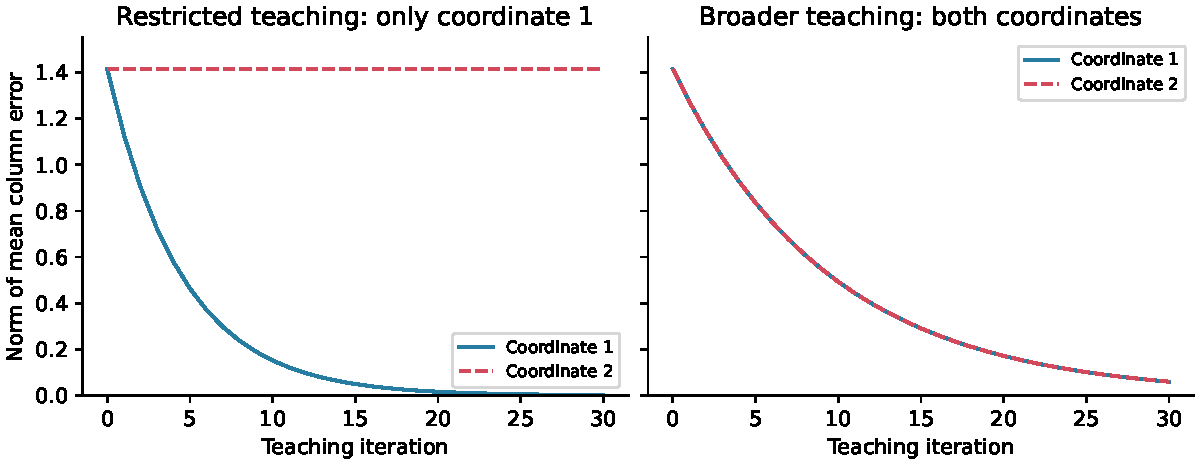
\includegraphics[width=.88\linewidth]{figure_learning_example.pdf}\caption{Worked learning example. Restricted teaching repairs only the excited column. Broader teaching contracts both columns in mean. Each initial column-error norm is $\sqrt{2}$. Curves are norms of the mean column errors, not mean-square or individual-trajectory stability claims.}\label{fig:learningexample}\end{figure}

\section{Synthetic checks and competing predictions}\label{sec:simulation}
\subsection{Reciprocal projection and latency checks}\label{sec:reciprocal-checks}
The new fixed-gate examples are implemented in \texttt{simulate\_reciprocal.py}, with all amplitudes and event times saved in \texttt{reciprocal\_results.json}. The invariant-channel example reaches threshold 0.34 at 78 ms, compared with a direct arrival at 18 ms; neither the reverse-path removal nor a threshold equal to the asymptotic limit produces finite completion. Two nonzero diagonal maps have a zero item-specific return. Compensating the two edge delays by 4 ms and $-2$ ms preserves the complete 8 Hz carrier response to within $9\times10^{-17}$, while moving onset and echo times. The independent verifier additionally compares the matrix echo series with direct time-stepped recurrence for 100 random stable map pairs, checks signed cancellation, and verifies the threshold regimes against a separately calculated partial sum. These checks establish implementation and conditional predictions; parameters are supplied, not recovered from neural data.
The supplement gives equations, seeds, trial counts, exact feature sets, and executable checks. The revised experiments and original supplied simulations are separately labeled. Identity checks test implementation; recovery and rival comparisons test statistical consequences within the stated synthetic designs.

\subsection{Delayed dictionaries and interaction memory}\label{sec:delayresults}
A comparator that includes the generating delayed product predicts almost as well as the delayed bilinear model. The experiment therefore demonstrates the effect of available features on prediction, rather than unique mechanism identification.
The supplied delayed generator uses 5 ms sampling and disjoint chronological training, validation, and test partitions. Validation selects the imposed 10 ms and 30 ms interaction lags. A rerun gives test MSE 0.001907 for an additive model, 0.002017 for an instantaneous bilinear model, 0.002062 for an instantaneous quadratic excluding the delayed product, 0.000415 for the delayed bilinear model, and 0.000418 for a quadratic including that same delayed product. Thus the apparent advantage depends on the rival's features; a flexible model containing the generating term predicts equally well. Maps and kernels are supplied. The factorial identity agrees to $1.7\times10^{-16}$. It confirms implementation, not biological mechanism.

\paragraph{Uncertainty of the prediction comparison.} A new comparison reruns the complete generator, validation selection, refitting, and untouched test evaluation in 300 independent series (seed 402600). Every series contains 900 samples; the usable partitions have 500 training, 150 validation, and 220 test samples. Models are paired within each realization, so correlated samples within a series are not treated as independent inferential replicates. The difference is rival MSE minus delayed-predictor MSE. Table~\ref{tab:mse-ci} reports its mean and pointwise Student-$t$ 95\% interval across realizations; four two-sided tests are adjusted by Holm's method. Lag selection recovered the generating pair in all 300 realizations.

\begin{table}[htbp]\centering\small
\caption{Paired test-risk differences over 300 independent synthetic realizations (seed 402600). Positive values favor the delayed bilinear predictor. Differences and confidence limits are in $10^{-3}$ squared output units. Intervals are pointwise 95\%; the four two-sided tests use Holm adjustment.}\label{tab:mse-ci}
\begin{tabularx}{\linewidth}{@{}Yrrr@{}}\toprule
Rival & Mean difference & 95\% interval & Adjusted $p$\\\midrule
Additive & 1.49090 & [1.41112, 1.57067] & $<10^{-6}$\\
Instantaneous bilinear & 1.50419 & [1.42383, 1.58455] & $<10^{-6}$\\
Quadratic without delayed product & 1.51213 & [1.43155, 1.59270] & $<10^{-6}$\\
Quadratic with delayed product & 0.00130 & [0.00094, 0.00165] & $<10^{-6}$\\
\bottomrule\end{tabularx}\end{table}

The mean advantage over the quadratic containing the delayed product is $1.30\times10^{-6}$, with interval $[0.94,1.65]\times10^{-6}$. It is statistically detectable in this Monte Carlo experiment but approximately three orders of magnitude smaller than the advantage over feature-omitting rivals. No practical-equivalence test or neural population inference is claimed. The uncertainty describes expected prediction risk under this synthetic generator, not an empirical confidence interval for a biological mechanism.

\subsection{Nervous-network arrival and dispersion checks}\label{sec:nervous-checks}
The added verifier uses seed 6102026. Across 100 independently generated four-population networks with two features per population, a direct method-of-steps implementation agrees with an independently iterated retarded-operator series to maximum absolute error $8.9\times10^{-16}$. Each edge has a nonnegative normalized three-point processing measure and a positive discrete conduction delay. Randomized checks test the dispersion and signed threshold bounds in 2,000 cases each. The 8 ms route in Figure~\ref{fig:nervous-network} is null for the tested item; a supported detour first appears at 12 ms. Opposing simultaneous routes cancel despite their nonzero individual coefficients. With a shared 15 ms processing mean, uniform half-widths of 2 and 10 ms give 40 Hz temporal magnitudes 0.958 and 0.234. These numbers check the specified operators and bounds. They do not estimate axonal speeds or population maps from neural data. Supplement S19 specifies the complete reproduction contract.

\subsection{Coupling recovery with matched observed features}\label{sec:recovery}
The original exact-feature experiment covered truth in 52 of 60 nominal 95\% intervals. Correlation between included regressors is already accounted for by OLS covariance and is not, by itself, a valid explanation of undercoverage. Sixty realizations cannot precisely estimate coverage, and no causal diagnostic is claimed for the original discrepancy.
A revised experiment uses 2,000 independent realizations, 500 observations per realization, true coupling 0.6, and Gaussian residual SD 0.02. The mean coupling estimate is 0.59936 (between-run SD 0.01369). Normal intervals cover in 1,897/2,000 runs (94.85\%) and Student-$t$ intervals in 1,900/2,000 (95.00\%). With independent feature noise SD 0.15, nominal Student-$t$ coverage is 47/2,000 (2.35\%) and the coupling mean falls to 0.33564. This is an errors-in-variables failure of the naive fitted model.
A 2,000-resample pairs bootstrap on the first 60 exact-feature realizations covers 57/60 (95\%; Wilson interval 86.30--98.29\%). Its small number of coverage trials does not establish superiority over analytic intervals, which also cover 57/60 on that subset. No unrun approximate bootstrap coverage is reported.

\begin{figure}[htbp]\centering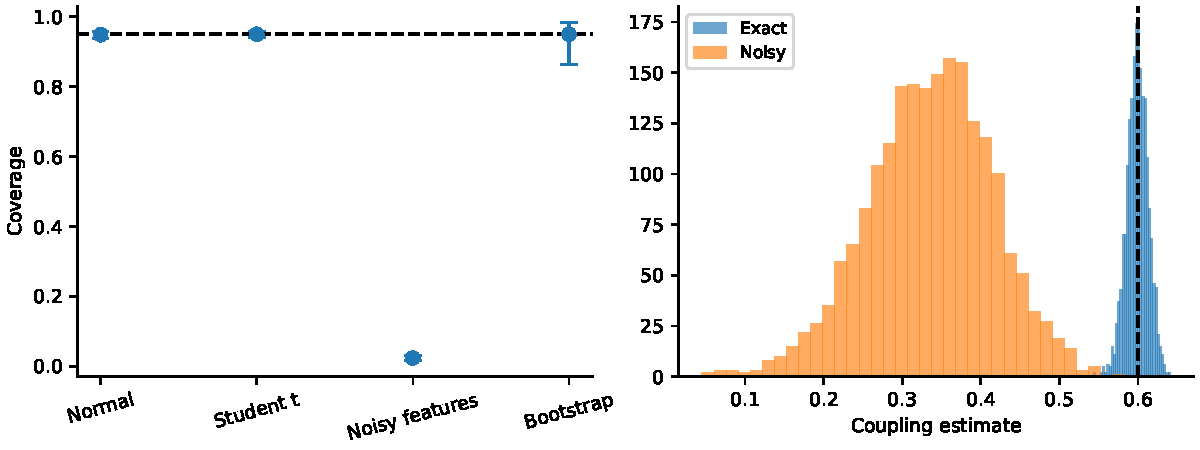
\includegraphics[width=.9\linewidth]{figure_coverage.pdf}\caption{Revised interval experiment. Exact measured features support nominal coverage under the correct Gaussian regression model; adding feature error makes the naive estimator biased and its intervals severely misleading.}\label{fig:coverage}\end{figure}

\section{Practical recovery under source mixing}\label{sec:practical}
Stylized 8~Hz sensors, sampled at 250~Hz, are passed through an ideal 6--10~Hz cutoff. This is not a lead-field model. At the scripted noise levels, clean 10~dB phase RMSE is \CleanTenRmse{}~rad with $\widehat\kappa=\CleanTenKappa$; mixing at 0~dB is \MixZeroRmse{}~rad, $\widehat\kappa=\MixZeroKappa$; common drive at 0~dB is \DriveZeroRmse{}~rad, $\widehat\kappa=\DriveZeroKappa$; both are \MixdriveZeroRmse{}~rad, $\widehat\kappa=\MixdriveZeroKappa$. The imposed harmonic is at 16~Hz, outside the ideal 6--10~Hz analysis band. The filter therefore removes it completely, reducing the harmonic-alone condition to clean 0~dB. This is a property of this filter, not evidence that harmonics are generally harmless. An alternative generator $y=0.55+0.35\cos(2\delta)+\zeta$ prefers the gate over a constant in \FalseConst/24 runs and over Fourier in \FalseFourier/24. Mean MSEs are \AltGate{}, \AltConst{}, and \AltFourier{}. Structural identifiability does not imply recovery from a sensor mixture. Mixing plus common drive moves fitted concentration from about \CleanTenKappa{} to about \MixdriveZeroKappa{}. The ideal 6--10~Hz filter removes the imposed harmonic and is not a lead field. The retained plot is Supplementary Figure~S4.

\paragraph{Interpretation.} The retained sensor checks use the supplied original scripts, not a physiological lead field. Their filtered harmonic condition cannot establish robustness to retained harmonics. Mixing and common input are recovery failures to be modeled, not evidence for a universal phase mechanism.

\section{Independent experiments and rejection criteria}\label{sec:experiment}
Use four independent stages: localize edges and target readouts; freeze maps, processing assumptions, thresholds, and gain calibration; estimate on separate data; test on untouched data. Randomize calibrated arrival-phase conditions and sham controls while matching content and power. Check that intervention changes the intended phase and does not change the content code. Avoid outcome-selected ``unaware'' trials \citep{shanks2017}.

\begin{table}[htbp]\centering
\caption{Tests of specified model components after successful independent calibration and manipulation checks.}\label{tab:reject}
\begingroup\setlength{\tabcolsep}{5pt}\renewcommand{\arraystretch}{1.2}\hyphenpenalty=10000
\begin{tabularx}{\linewidth}{@{}>{\RaggedRight\arraybackslash}p{.33\linewidth}Y@{}}\toprule
Assumption checked & Contradicting outcome\\\midrule
Isolated fixed map; zero readout projection & Timing alone yields nonzero transfer in that readout.\\\addlinespace[5pt]
Known item: maximum amplitude $A_v<\theta$ & Posting occurs under the stated scalar gate and threshold.\\\addlinespace[5pt]
Positive downstream noise; calibrated channel gain & A confirmatory interval excludes the pilot-frozen sensitivity effect predicted by Eq.~\eqref{eq:sensitivity}.\\\addlinespace[5pt]
Fixed matched inputs; separable model & A reproducible nonzero factorial contrast rejects separability. It does not exclude every joint readout alternative.\\\addlinespace[5pt]
Learning opportunity assigned zero & A reproducible item-specific map change contradicts Eq.~\eqref{eq:plastic}.\\\addlinespace[5pt]
Two bands; shared transfer phase; known processing & Offset data contradict the shared-phase response after allowing for phase aliases and uncertainty.\\\addlinespace[5pt]
Isolated reciprocal paths; independently resolved returns & A matched reverse-path manipulation changes the initial forward increment while all forward inputs and parameters remain fixed, contradicting Eq.~\eqref{eq:echo}.\\\addlinespace[5pt]
Positive invariant channel; known timing and threshold & Held-out completion times contradict Eq.~\eqref{eq:recurrence-latency} beyond calibrated uncertainty.\\\bottomrule
\end{tabularx}\endgroup\end{table}
An uncontrolled mixture is an inconclusive identifying experiment, not a mathematical rejection of the ridge. A null interaction test needs precision against a meaningful effect bound. Content projection, gain, criterion, and alternative pathways must be measured or constrained independently.

\subsection{Public datasets and a staged empirical route}\label{sec:publicdata}
Public CCEP dataset ds004080 provides controlled single-pulse stimulation, event timing and atlas-labeled electrode positions \citep{vanblooijs2023,ccepdata}. We retrieved and screened all 74 electrode metadata tables from its NEMAR v1.0.0 mirror. Only one table has explicit contacts in both hemispheres; its single frontal-name label is on the left, with no frontal-name labels on the right. This identifies a candidate for anatomical and stimulation-coverage inspection, not validated bilateral prefrontal sampling. Evoked response onset and peak must also be separated from artifact and processing before being interpreted as conduction.

Allen Visual Coding Neuropixels is a candidate for held-out population projection and lagged transfer, while Visual Behavior Neuropixels additionally supplies a task and behavioral events \citep{allencoding,allenbehavior}. These observational datasets do not by themselves supply the isolated two-source factorial intervention or a known phase-gain manipulation. F-TRACT's derived maps offer a possible independent delay reference, subject to model assumptions and access checks \citep{ftractatlas}. Supplement S16, its expanded dataset comparison, and the accompanying data review specify sources, versioning, actual metadata screening, and the remaining design gaps.

Additional releases improve individual component matches. The hippocampal--retrosplenial dataset associated with \citet{gonzalez2026} provides simultaneous populations and task/replay epochs for conditional subspace analyses. The multiplexed-subspace study of \citet{macdowell2025} includes frontal and other populations and explicitly concerns functional correlation rather than causal direction. DANDI 000458 combines timed cortical stimulation with EEG and Neuropixels in awake and anesthetized mice \citep{claar2023}; IBL's brain-wide decision-task release adds broad anatomical coverage and choices \citep{ibl2025data}. None supplies a documented two-band receptive scan, isolated reciprocal content perturbations, and the learning intervention jointly. These are candidates for separate falsifiable tests, not combined empirical confirmation.

The proposed empirical sequence is to test timing with controlled perturbations, estimate content maps and noise-whitened innovation on separate population recordings, and test behavior on independently held-out trials. These complementary datasets cannot be merged into one calibrated causal loop across species or cohorts. No inspected resource is asserted to validate all parts of the model, and no neural waveform was fitted in this revision.

\subsection{A minimal identifying experiment and precision planning}\label{sec:minimal}
The smallest targeted experiment tests the shared-phase observation model, rather than every extension at once. Independently establish a coarse delay branch, record calibrated carrier offsets at two distinct frequencies, and scan receptive gain at one frequency with matched content and power. Fit $\gamma,\alpha,\tau$ using the two carrier offsets and the receptive offset. Predict an independently measured onset latency after separately accounting for processing. A discrepancy beyond the frozen uncertainty rejects the shared transfer/processing assumptions or the observation channel. A single band supplies an equivalence class, so there is no uniquely defined single-band delay estimator whose systematic bias must be demonstrated to confirm the ridge.

For fixed known amplitude and concentration, one probe away from the stationary points of the gate has nonzero local receptive information. This mathematical minimum is a poor practical design: an unknown gate amplitude can confound it. Use several phases spanning both sides of the center, reserve phases for held-out prediction, and estimate nuisance parameters jointly. The supplied illustration uses 48 scan phases, 32 independent phase trials per frequency, and two frequencies; these are generator choices, not established biological minima. Computing a two-band offset fit is constant-size linear algebra; a nonlinear fit with $N$ probe observations costs $O(N)$ per residual/Jacobian evaluation for a fixed number of parameters. No algorithmic complexity advantage is claimed.

\paragraph{Timing precision is not an electrode count.} For independent latency estimates with standard deviation $\sigma_\tau$, a normal-approximation 95\% mean-interval half-width $e$ requires $N\gtrsim(1.96\sigma_\tau/e)^2$. With illustrative $\sigma_\tau=3$ ms and $e=1$ ms, this is 35 independent estimates. Repeated pulses and nearby electrodes need not be independent; subject-level uncertainty requires subjects or a justified hierarchical model. At least one valid stimulus site and a recorded target are necessary for a directed timing test, and both directional interventions are needed for reciprocity. There is no universal number of electrodes per hemisphere that ensures delay precision. Spatial coverage, artifacts, sampling, pulse variability and indirect routes determine eligibility and effective information. Estimate these from pilot waveforms before freezing sample size.

\paragraph{Factorial contrast precision.} For a prespecified scalar receiver contrast, equal independent cell sizes $n$ and within-cell variance $\sigma^2$ give variance $4\sigma^2/n$ for the four-cell difference. To detect magnitude $D$ with power $1-\beta$ using $K$ prespecified two-sided contrasts and a Bonferroni family bound $\alpha_0$,
\begin{equation}
n\gtrsim\frac{4\sigma^2}{D^2}
\left[z_{1-\alpha_0/(2K)}+z_{1-\beta}\right]^2,
\label{eq:factorial-power}
\end{equation}
where $z_p$ is the standard normal quantile. For $K=4$, $\alpha_0=0.05$, power 0.8, and $D/\sigma=0.5$, this gives 179 trials per cell. It is a planning illustration for independent Gaussian contrasts, not a recommendation for Allen recordings. Ordinary stimulus classes are not automatically the four independent pathway interventions required by the factorial theorem.

The number of basis pairs is $r_1r_2$, but rank detection also depends on the smallest nonzero singular value and uncertainty in maps, whitening, and contrasts. A single nonzero scalar contrast does not identify rank. If a simultaneous calibration supplies $\|\widehat{QC_B}-QC_B\|_2\le e_C$ with its declared confidence, singular-value perturbation bounds give $\sigma_j(\widehat{QC_B})>e_C$ as evidence that the true $j$th singular value is positive on that event. An observed value below $e_C$ is unresolved, not evidence of an exact null. Pilot cluster resampling and held-out null controls must determine $e_C$ and the achievable effect bound.

\paragraph{Decisive component tests.} Test identifying assumptions by predicting independent timing; test content delivery with an independently calibrated sender contrast at matched phase; test returns by changing the reverse pathway while checking that the initial forward increment is unchanged; and test learning by training one content subspace and evaluating an orthogonal held-out direction. Nonzero projection without threshold crossing and two nonzero maps without an item return are predicted failure cases, not falsifications. Failure to reach statistical significance alone does not reject a model: an exclusion interval against a prespecified meaningful effect is required.

\subsection{A nervous-system test: content support versus total arrival time}\label{sec:nervous-test}
A particularly relevant public candidate is the release accompanying \citet{michaels2025}. Its Dryad description lists session-level spike timing, hand and joint kinematics, and trial timing and conditions, with a recording-session information table \citep{michaelsdata2025}. The experiment uses mechanically perturbed sensorimotor behavior and neural population recordings. It can support an initial held-out test of whether matched perturbation contrasts occupy different receiver readouts and arrive at different times. Mechanical perturbation is a timed sensory input, not a selective intervention on an isolated cortical edge.

\paragraph{What the release actually covers.} A fresh audit of the official Dryad version manifest identifies 49 session files (29 from monkey M and 20 from monkey P). The paper's Extended Data Table 1 provides a more restrictive eligibility screen: among S1, M1, PMd, and dlPFC, there are nine sessions with both PMd and dlPFC, three with S1 and M1, two with M1 and PMd, and two with S1 and PMd. These are simultaneous-area candidates, not 49 independent source--receiver pairs. No listed session pairs dlPFC directly with M1. Several PMd--dlPFC sessions contain very few PMd neurons, so a frozen minimum-feature/quality screen may reduce the nine eligible sessions further. The transcribed area-pair table and official file manifest accompany the code. Raw trial synchrony and preprocessing still require file-level verification; metadata-file download endpoints returned access errors in this audit, and no new waveform fit was performed.

The proposed analysis first freezes the source and receiver features, readouts, preprocessing delays, and training/test split. Next it compares three models on identical held-out trials: (a) a common scalar delay with fixed projection; (b) content-specific projected routes with their independently constrained delays; (c) a flexible delayed nonlinear predictor using the same inputs. A success for (b) must predict both a selective near-null contrast and the later supported contrast, improve paired held-out error with session-level uncertainty, and survive the flexible rival. Inferring routes additionally requires simultaneous source--target coverage and controlled alternatives. Session metadata must establish that coverage before any paired-population model is fitted. Conditioning on movement or trial outcome can itself bias interpretation.

A decisive perturbation of the proposed detour would change its later response while preserving an independently supported early route. A paired-site peripheral stimulation study is a complementary timing calibration: subtracting proximal and distal onset times can cancel shared downstream stages under a justified common-path model. It does not identify a content translation from muscle voltage alone. The open PhysioNet EMG examples contain voluntary muscle recordings, rather than synchronized paired-site conduction stimulation and source/receiver population contrasts \citep{emgexamples2009}; they are therefore unsuitable for testing the complete model. F-TRACT's downloadable derived atlas adds a model-dependent latency reference \citep{ftractzenodo2022}, not independently calibrated content maps. None of these resources alone identifies the entire nervous-system network, its receptive phase, its interaction rank, and its learning rule.

No additional biological waveform was fitted in this revision. The prospective contribution is the jointly calibrated prediction in Theorem~\ref{thm:network}, not retrospective agreement obtained by interpreting any observed latency as its delay term. Sample planning must use independent-session variance and the number of tested source contrasts; repeating dense within-trial time points does not increase biological replication.

\paragraph{Concrete planning and rejection.} Let $D_s$ be the held-out MSE of a rival minus that of the projected-route model in independent replication unit $s$, and $d=\mathbb E D_s/\operatorname{SD}(D_s)$. For two prespecified rival comparisons, use two-sided level $0.025$ each (Bonferroni familywise level $0.05$). Under normal independent unit-level differences, exact noncentral-$t$ planning gives:
\begin{center}\begin{tabular}{@{}ccc@{}}\toprule
Assumed standardized advantage $d$ & Units for 80\% power & Units for 90\% power\\\midrule
0.3 & 109 & 141\\
0.5 & 41 & 53\\
0.8 & 18 & 23\\\bottomrule
\end{tabular}\end{center}
These are assumed-effect calculations, not estimates from the release. Achieving 90\% power for each comparison guarantees at least 80\% joint power by the union bound. Freeze a practically meaningful MSE margin as well as the comparisons; a tiny significant improvement is insufficient. Repeated sessions from the same animal require clustering, and neurons and time bins are not independent replication units. Two animals cannot establish population-level uncertainty across animals from session count alone.

A selective near-null prediction needs an equivalence test rather than a nonsignificant response. As a concrete planning illustration, two one-sided tests at level $0.025$, a margin of $0.3$ unit-level response SD, true mean zero, and independent normal contrasts require 119 units for 80\% equivalence power or 147 for 90\%. These values integrate over the estimated sample variance, rather than treating it as known. Prespecify an early window, a null contrast, a supported contrast, and a minimum late-response amplitude from independent calibration. Joint confirmation requires the early contrast within its equivalence margin and the later contrast above its positive-effect bound; correct for any additional contrasts or windows. These planning assumptions may be unattainable in this release, which would make it exploratory for the joint claim.

With adequate calibration and precision, an early-response confidence interval excluding the predicted near-null range, a late-response upper confidence bound below the calibrated minimum, or timing inconsistent with the independently constrained route excludes the fitted route hypothesis. Failure to outperform a flexible rival limits predictive usefulness; it does not by itself disprove the algebraic network theorem. Without resolved source--receiver coverage or enough independent replication, the result is inconclusive. Supplement S20 and \texttt{verify\_revision\_planning.py} reproduce these calculations.


\section{Discussion}\label{sec:discussion}
\subsection{What the phase score can identify}
The explicit observation separates carrier phase $\gamma$ from receptive center $\alpha$. One band identifies at most their effective offsets, leaving an exact compensating delay direction. Phase-only data identify the carrier offset and do not establish receiver preference. Shared transfer phase across two frequencies plus a gain scan provides a constructive local escape. Harmonic rank depends on response constraints; common drive requires a valid complex-signal observation model.

\subsection{Support, delivery, and completion}
Theorem~\ref{thm:inter} establishes modeled interregional communication when the item has nonzero readout projection: a sender-dependent receiver contribution exists, and a projected source contrast changes that contribution at matched phase. Structural support is readout nonorthogonality to the translation image. Item-specific delivery requires nonzero $v^\top Mz$. Neither guarantees threshold feasibility or finite completion. The positive gate attenuates at every phase, including $\pi$. Completion is a declared operational first-passage measure, and a transient conduction onset is not invariant merely because carrier phase is compensated. The retained two-stage account therefore separates support from effectiveness without claiming that projection alone explains report delays.

\subsection{The link between identification and delivery}
The reciprocal extension supplies a common input--output object, rather than a rhetorical dependence between otherwise separate theorems. Its frequency-domain response and time-domain return series use the same directed map products. The stationary likelihood constrains effective gate and carrier offsets; the return-product theorem constrains which projected perturbations can circulate; resolved content onsets and echoes add a transverse timing measurement. Equation~\eqref{eq:recurrence-latency} then predicts an operational waiting term from an independently calibrated positive channel. It does not manufacture an unmeasured physiological delay. The zero-return example shows that two individually nonzero maps need not support the item's round trip.
The shared gate offset connects the two levels. It creates a conditional amplitude equivalence, while independent onset observations can break a carrier equivalence. Testing delivery does not require recovering every internal parameter. Testing a physiological explanation for delivery does require calibrated constraints on delay, transfer phase, receptive center, and noise. The sensitivity result is derived from the explicit behavioral readout, not from geometry alone.

\paragraph{Formal relationship to neighboring methods.} The distinction is between what each observation constrains and what further assumptions permit inference.
\begin{table}[htbp]\centering\small
\caption{Measurement constraints and the additional inference made here.}\label{tab:formal-comparison}
\begin{tabularx}{\linewidth}{@{}p{.24\linewidth}YY@{}}\toprule
Approach & What it constrains & Additional requirement\\\midrule
Phase-slope index \citep{nolte2008} & Frequency-dependent cross-spectral phase and a directional summary & A physiological delay interpretation requires constrained transfer and processing phases.\\\addlinespace
Delay/interference analysis \citep{dowdall2023} & Effects of delays on coherence and Granger estimates in interacting systems & The present ridge concerns an explicit conditional carrier/gate likelihood, not the same interference mechanism.\\\addlinespace
Communication subspaces \citep{semedo2019} & Predictive population directions across areas & A causal pathway and a threshold/readout rule require independent calibration and interventions.\\\addlinespace
This model & Offset equivalence, projected item contrasts, return products and operational first passage & Known observation channels, constrained phase branches, calibrated maps, and module-specific tests.\\\bottomrule
\end{tabularx}\end{table}
Granger causality assesses whether past signals improve prediction within a specified multivariate time-series model. Broadband lag structure can add information beyond the stationary one-band carrier observation; the ridge does not prove that all Granger analyses are uninformative. Conversely, a selected predictive lag is not automatically an anatomical conduction time, particularly under feedback, unknown filtering, or omitted inputs. The empirical comparison should fit those rival time-series explanations to the same held-out perturbation responses, rather than infer a delay from a single summary.


\subsection{Relation to existing accounts}
Recent studies already link population geometry to interregional activity and contextual actions \citep{macdowell2025,gonzalez2026,binish2026}. Projection alone is therefore not the novelty claim; the prospective advance is a calibrated joint test separating offset recovery, item delivery, and return-dependent first passage. The gate is compatible with communication-through-coherence \citep{fries2015}; its presence is not established by a phase--report correlation. Translation support complements communication-subspace ideas \citep{semedo2019}. The exact parameter equivalence is distinct from the delay-dependent interference mechanism analyzed by \citet{dowdall2023}; both caution against assigning a unique physiological meaning to a phase summary. Report-status labels do not distinguish theories of experience \citep{dehaene2006,lamme2006}. The factorial experiment distinguishes a cross-path term from separable alternatives, but joint nonlinear readouts remain viable. The model's scientific value lies in these precise contrasts and failure cases rather than an unsupported claim of a breakthrough.

\subsection{Beyond a two-population loop}
Theorem~\ref{thm:network} makes the same projection and delay architecture usable for multistage signaling. Its distinctive test separates the fastest anatomical route from the fastest route supporting a specific decoded contrast. Parallel signed routes can suppress an observed response, and dispersed processing can reduce carrier magnitude despite intact content support. Proposition~\ref{prop:dispersion} also limits interpretation: even a complete temporal response cannot separate conduction from a causal processing kernel whose support can be shifted. A claimed missing nervous-system delay must therefore be measured or independently constrained. These statements strengthen the model's experimental consequences; the walk expansion and Fourier bound are classical methods, so mathematical or biological priority is not established here.

\subsection{A unified experimental opportunity}
The useful research opportunity is to distinguish four failure modes that can produce similar low-report outcomes: an unsupported item, weak receptive gain, missing cross-path contribution, and unlearned translation. They make different predictions. Phase tuning cannot restore an exactly null item projection. Better alignment can increase a supported item's amplitude without changing the content span. A bilinear contribution can add a receiver direction outside the additive span, measurable through complement factorial contrasts. Learning can reduce translation error only in the gain-weighted excited subspace under the stated update.

A combined experiment should therefore freeze content maps and their uncertainty, recover timing offsets using the calibrated design, randomize projected content contrasts at matched inputs, estimate the complement rank with held-out basis pairs, and test transfer after training on restricted versus broader content sets. These are proposed empirical stages, not completed neural results. A decisive finding would be successful out-of-sample prediction of which receiver directions appear, their gain dependence, and their change after restricted training. A failure after valid calibration would identify which model component needs replacement.

The potential advance is a measurable separation of support, timing, nonlinear integration, and learning in the same independently calibrated pathway. Claims of biological novelty or a breakthrough require experimental evidence and a focused comparison with existing theories. Renaming the model's definitions cannot supply that evidence.

\subsection{Limits and the next step}
All evidence here is synthetic. Correct-model recovery, valid coverage, and algebra checks establish implementation and internal consequences. They do not establish a neural mechanism, a learning rule, or a consciousness account. The next empirical step is independent calibration of a content map and readout followed by a matched-input gain manipulation, alongside latency or multi-frequency measurements if physiological parameter separation is sought.

\subsection*{Transparency}\label{sec:transparency}
\funding{This research received no external funding.}
\conflicts{The author declares no conflict of interest.}
\dataavailability{All observations are synthetic. The accompanying package contains revised results, original supplied outputs retained for provenance, and a supplementary protocol with independently runnable checks. Public electrode and event metadata were screened for feasibility; no neural waveform or behavioral trial data were fitted to the model.}
\codeavailability{Public project code: \url{https://github.com/lolzguycoder/esj-phase-connectivity}. Project archive DOI supplied by the author: \href{https://doi.org/10.5281/zenodo.23165931}{10.5281/zenodo.23165931}. The accompanying revision includes the complete manuscript source, supplement, \texttt{model.py}, \texttt{simulate.py}, \texttt{simulate\_reciprocal.py}, \texttt{verify\_nervous\_network.py}, \texttt{verify.py}, \texttt{reproduce.py}, pinned requirements, numerical outputs, and figures. Correspondence of the cited archive to this exact revised package has not been independently verified. Reproduction instructions are in the supplement and \texttt{README.md}.}
\authorcontributions{Karem Abdelgalil: conceptualization, formal analysis, software, and writing.}


\bibliography{references}
\end{document}
